\documentclass[12pt,a4paper]{report}


\usepackage[utf8]{inputenc} % pentru suport diacritice
\usepackage[english]{babel} % setări pentru limba română 
\renewcommand\familydefault{\sfdefault} % sans serif

\usepackage[margin=2.54cm]{geometry}	% dimensiuni pagină și margini
\usepackage{graphicx} % support the \includegraphics command and options
\graphicspath{ {./img/} }

% formatting sections and subsections
\usepackage{textcase}
\usepackage[titletoc, title]{appendix}
\usepackage{titlesec}
\titleformat{\chapter}{\large\bfseries\MakeUppercase}{\thechapter}{2ex}{}[\vspace*{-1.5cm}]
\titleformat*{\section}{\large\bfseries}
\titleformat*{\subsection}{\large\bfseries}
\titleformat*{\subsubsection}{\large\bfseries}

\usepackage{chngcntr}
\counterwithout{figure}{chapter} % no chapter number in figure labels
\counterwithout{equation}{chapter} % no chapter number in equation labels

\usepackage[table,xcdraw]{xcolor}
\usepackage{sectsty}
\chapterfont{\color{black}}  % sets colour of chapters
\sectionfont{\color{black}}  % sets colour of sections

\usepackage{booktabs} % for much better looking tables
\usepackage{url} % Useful for inserting web links nicely
\usepackage[bookmarks,unicode,hidelinks]{hyperref}


\usepackage{array} % for better arrays (eg matrices) in maths
\usepackage{paralist} % very flexible & customisable lists (eg. enumerate/itemize, etc.)
\usepackage{verbatim} % adds environment for commenting out blocks of text & for better verbatim
\usepackage{subcaption} 
\usepackage{enumitem}
\usepackage{adjustbox}

\usepackage{amsmath}
\usepackage{amsfonts} 
\usepackage{amsthm} 
\usepackage[ruled]{algorithm}
\usepackage{algpseudocode}
\usepackage{enumitem}   


%jsons
\usepackage{listings}

\colorlet{punct}{red!60!black}
\definecolor{background}{HTML}{EEEEEE}
\definecolor{delim}{RGB}{20,105,176}
\colorlet{numb}{magenta!60!black}

\lstdefinelanguage{json}{
    basicstyle=\normalfont\ttfamily,
    numbers=left,
    numberstyle=\scriptsize,
    stepnumber=1,
    numbersep=8pt,
    showstringspaces=false,
    breaklines=true,
    frame=lines,
    backgroundcolor=\color{background},
    literate=
     *{0}{{{\color{numb}0}}}{1}
      {1}{{{\color{numb}1}}}{1}
      {2}{{{\color{numb}2}}}{1}
      {3}{{{\color{numb}3}}}{1}
      {4}{{{\color{numb}4}}}{1}
      {5}{{{\color{numb}5}}}{1}
      {6}{{{\color{numb}6}}}{1}
      {7}{{{\color{numb}7}}}{1}
      {8}{{{\color{numb}8}}}{1}
      {9}{{{\color{numb}9}}}{1}
      {:}{{{\color{punct}{:}}}}{1}
      {,}{{{\color{punct}{,}}}}{1}
      {\{}{{{\color{delim}{\{}}}}{1}
      {\}}{{{\color{delim}{\}}}}}{1}
      {[}{{{\color{delim}{[}}}}{1}
      {]}{{{\color{delim}{]}}}}{1},
}
%end of jsons



\newtheorem{theorem}{Theorem}[section]
\newtheorem{corollary}{Corollary}[theorem]
\newtheorem{lemma}[theorem]{Lemma}
\newtheorem{definition}{Definition}[section]
\newtheorem*{remark}{Remark}

\newtheorem{pitfall}{Pitfall}[theorem]
\newtheorem{fallacy}{Fallacy}[theorem]


\setlist{noitemsep}

%%% HEADERS & FOOTERS
\usepackage{fancyhdr}
\pagestyle{empty}
\renewcommand{\headrulewidth}{0pt}
\renewcommand{\footrulewidth}{0pt}
\lhead{}\chead{}\rhead{}
\lfoot{}\cfoot{\thepage}\rfoot{}
\newcommand{\alg}{\texttt{algorithmicx}}
\newcommand{\old}{\texttt{algorithmic}}
\newcommand{\euk}{Euclid}
\newcommand\ASTART{\bigskip\noindent\begin{minipage}[b]{0.5\linewidth}}
\newcommand\ACONTINUE{\end{minipage}\begin{minipage}[b]{0.5\linewidth}}
\newcommand\AENDSKIP{\end{minipage}\bigskip}
\newcommand\AEND{\end{minipage}}

\renewcommand{\qedsymbol}{\rule{0.7em}{0.7em}}



\newcommand{\HeaderLineSpace}{-0.25cm}
\newcommand{\UniTextRO}{UNIVERSITATEA POLITEHNICA DIN BUCUREȘTI \\[\HeaderLineSpace] 
FACULTATEA DE AUTOMATICĂ ȘI CALCULATOARE \\[\HeaderLineSpace]
DEPARTAMENTUL DE CALCULATOARE\\}
\newcommand{\DiplomaRO}{PROIECT DE DIPLOMĂ}
\newcommand{\AdvisorRO}{Coordonator științific:}
\newcommand{\BucRO}{BUCUREȘTI}

\newcommand{\UniTextEN}{UNIVERSITY POLITEHNICA OF BUCHAREST \\[\HeaderLineSpace]
FACULTY OF AUTOMATIC CONTROL AND COMPUTERS \\[\HeaderLineSpace]
COMPUTER SCIENCE AND ENGINEERING DEPARTMENT\\}
\newcommand{\DiplomaEN}{DIPLOMA PROJECT}
\newcommand{\AdvisorEN}{Thesis advisor:}
\newcommand{\BucEN}{BUCHAREST}

\newcommand{\frontPage}[6]{
\begin{titlepage}
\begin{center}
{\Large #1}  % header (university, faculty, department)
\vspace{50pt}
\begin{tabular}{p{6cm}p{4cm}}

\includegraphics[scale=0.8]{pics/upb-logo.jpg} &
	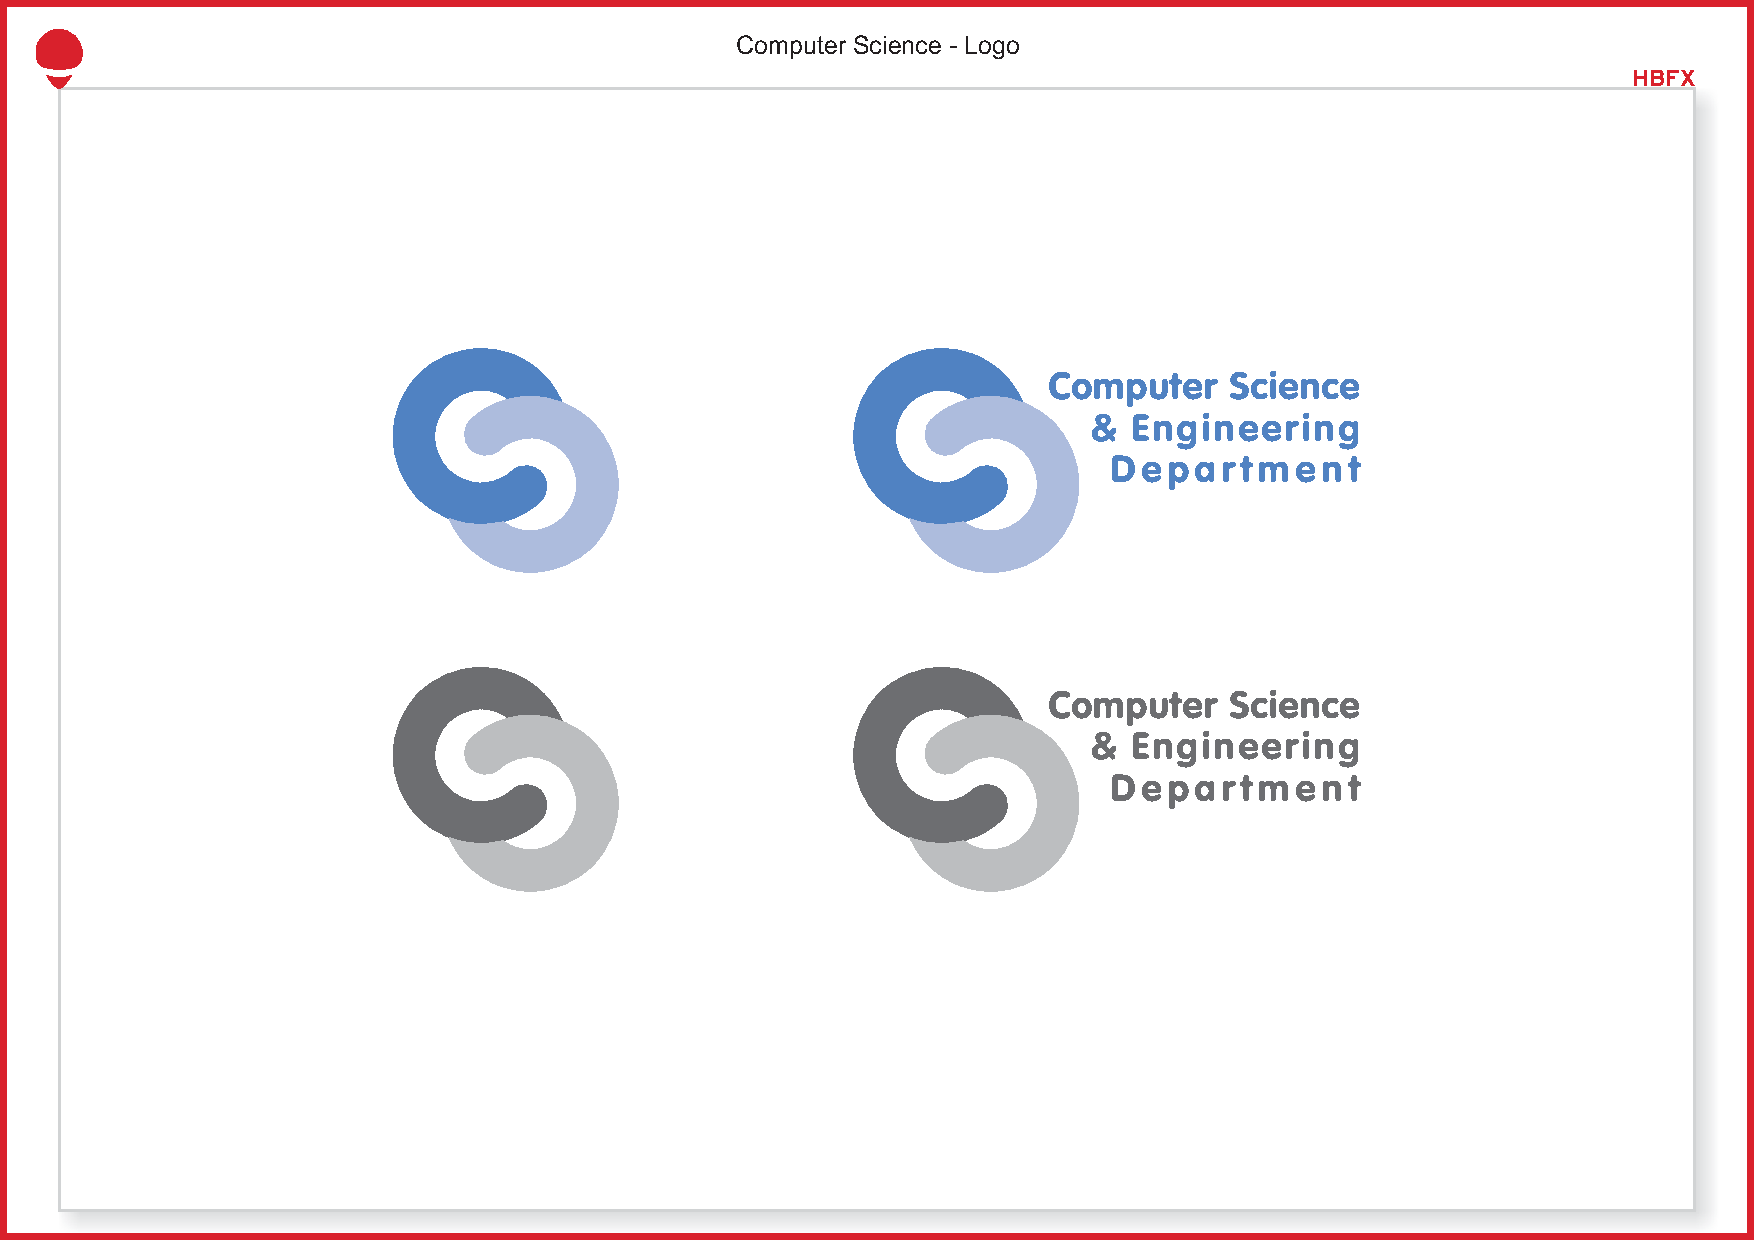
\includegraphics[scale=0.5,trim={14cm 11cm 2cm 5cm},clip=true]{pics/cs-logo.pdf}
\end{tabular}

\vspace{105pt}
{\Huge #2}\\                           % diploma project text
\vspace{40pt}
{\Large #3}\\ \vspace{0pt}  % project title
{\Large #4}\\                          % project subtitle
\vspace{40pt}
{\LARGE \Name}\\                   % student name
\end{center}
\vspace{60pt}
\begin{tabular*}{\textwidth}{@{\extracolsep{\fill}}p{6cm}r}
&{\large\textbf{#5}}\vspace{10pt}\\      % scientific advisor
&{\large \Advisor}                                    % advisor name
\end{tabular*}
\vspace{20pt}
\begin{center}
{\large\textbf{#6}}\\                                % bucharest
\vspace{0pt}
{\normalsize \Year}
\end{center}
\end{titlepage}
}

\newcommand{\frontPageRO}{\frontPage{\UniTextRO}{\DiplomaRO}{\LARGE \ProjectTitleRO }{\small \ProjectSubtitleRO}{\AdvisorRO}{\BucRO}}
\newcommand{\frontPageEN}{\frontPage{\UniTextEN}{\DiplomaEN}{\LARGE \ProjectTitleEN}{\small \ProjectSubtitleEN}{\AdvisorEN}{\BucEN}}

\linespread{1.15}
\setlength\parindent{0pt}
\setlength\parskip{.28cm}

%% Abstract macro
\newcommand{\AbstractPage}{
\begin{titlepage}
\textbf{\large SINOPSIS}\par
\AbstractRO\par\vfill
\textbf{\large ABSTRACT}\par
\AbstractEN \vfill
\end{titlepage}
}




%%%%%%%%%%%%%%%%%%%%%%%%%%%%%%%%%%%%%%%%%%%%%%%%%%   
%%
%%          End of template definitions
%%   
%%%%%%%%%%%%%%%%%%%%%%%%%%%%%%%%%%%%%%%%%%%%%%%%%%


%%% Puteți elimina aceste linii din lucrare, servesc numai pentru template.
\newcommand{\worktype}[1]{[\textit{#1}] }
\newcommand{\dezvoltare}{\worktype{Dezvoltare de produs}}
\newcommand{\cercetare}{\worktype{Cercetare}}
\newcommand{\ambele}{\worktype{Ambele}}
%%%


%%
%%   Campurile de mai jos trebuie modificate de autor. Modificati doar continutul, nu si numele fiecarei definitii
%%
\newcommand{\ProjectTitleRO}{Metrici de evaluare a performanțelor și complexității pentru programele de calculatoare}
\newcommand{\ProjectSubtitleRO}{O noua abordare asupra modalitatilor traditionale de masurare a complexitatii algoritmilor si estimare a timpilor de rulare in raport cu arhitectura aleasa, in contextul infrastructurii dinamice}
\newcommand{\ProjectTitleEN}{Metrics for evaluating the performance and complexity of computer programs}
\newcommand{\ProjectSubtitleEN}{A new approach to the traditional ways of measuring the complexity of algorithms and estimating running times given the chosen architecture, in the context of dynamic infrastructure}
\newcommand{\Name}{Rares Folea}
\newcommand{\Advisor}{Prof. Emil-Ioan Slusanschi}
\newcommand{\Year}{2020}

% Setări document
\title{Proiect de diplomă}
\author{\Name}
\date{\Year}

%%
%%   Campurile aferente rezumatului
%%
\newcommand{\AbstractRO}{TODO}

\newcommand{\AbstractEN}{TODO}

\begin{document}

\frontPageRO
\frontPageEN

\begingroup
\linespread{1}
\tableofcontents
\endgroup

\AbstractPage


% Textul licentei incepe de aici 
\pagestyle{fancy}






\chapter{Classical Computational Complexity Calculus }


\section{Introduction}
This chapter will present the traditional methodology of calculus in the field of algorithm's computational complexity. The complexity will be expressed as a function $f:\mathbb{N}\longrightarrow\mathbb{R}$, where the function is characterized by the size of the input, while the evaluated value $f(n)$, for a given input size $n$, represents the amount of resources needed in order to compute the result. While the most often analyzed resource is time, expressed in elemental compute operations, the mathematical model is self-reliant for others natures of resources, including space reasoning or hybrid metrics. All the results of this chapter are well known in the literature and they represent the reference standard in calculating algorithm complexity in Computer Science. 

\section{Motivation}
Because of the difficulty of having a rigorous calculus of the complexity, an asymptotic computation approach for an algorithm's complexity offers a valuable insight about the real computational cost without requiring a precisely, flawless calculus.



\section{Family of Bachmann–Landau notations}
The following notations and names will be used for describing the asymptotic behavior of a algorithm's complexity characterized by a function, $f:\mathbb{N}\longrightarrow\mathbb{R}$. \\
We define the set of all complexity calculus $\mathcal{F}= \lbrace f:\mathbb{N}\longrightarrow\mathbb{R} \rbrace$
\\Assume that $n, n_{0}\in\mathbb{N}$. Also, we will consider an arbitrary complexity function $g \in \mathcal{F}$. \\

\begin{definition}
Assume that two continuous and derivable functions $v,w:\mathbb{R}\longrightarrow\mathbb{R}$ are considered to be similar in an \textbf{asymptotic analysis} iff: 
  \[\lim_{x\to\infty} \frac{v(x)}{w(x)} = c \in (-\infty, 0) \cup (0,\infty) \]
\end{definition}

\begin{corollary}
  Consider that if we analyses asymptotic behavior of functions defined over $\mathbb{N}$ the functions $v,w:\mathbb{N}\longrightarrow\mathbb{R}$ are similar iff there exists a function $r:\mathbb{N}\longrightarrow\mathbb{R}$, with $r(x) = \frac{v(x)}{w(x)}\ \forall\ x\in\mathbb{N}$, such that
  \[\lim_{x\to\infty} r(x) = \lim_{x\to\infty} \frac{v(x)}{w(x)} = C \in (-\infty, 0) \cup (0,\infty) \]
\end{corollary}

The following function classes can be therefore defined for any function $g:\mathbb{N}\longrightarrow\mathbb{R}$ that describes a convergent sequence or a divergent sequence with a limit that tends to infinity:
\begin{definition}   
  \textbf{Big Theta}: This set defines the group of mathematical functions similar in magnitude with  $g(n)$ in the study of asymptotic behavior. A set-based description of this group can be expressed as:
  \[\Theta(g(n))= \lbrace f \in \mathcal{F}\ |\ \exists c_{1}, c_{2} \in \mathbb{R}^{*}_{+}, \exists n_{0} \in \mathbb{N}^{*}\ s.t.\ \ c_{1} \cdot g(n) \leq f(n) \leq c_{2} \cdot g(n)\ ,\  \forall n \geq n_{0} \rbrace\]
\end{definition}  

\begin{corollary}
  Another useful method of establishing a Big-Theta relationship, if the composed sequence defined by the ratio of the two functions exists and also $ \lim_{x\to\infty} \frac{f(x)}{g(x)}$ exists, is by applying the sufficient condition:
    \[ f \in \Theta(g(n))\ \Leftrightarrow\ \lim_{x\to\infty} \frac{f(x)}{g(x)} = C \in (-\infty, 0) \cup (0,\infty) \]
\end{corollary}

Remark that  both $f,g$ can define divergent sequence with limits that tend to infinity, while the sequence $r(x) = \frac{f(x)}{g(x)}\ \forall\ x\in\mathbb{N}$ can be convergent and can have a nonzero limit. \\
Iff $ r(x) = \frac{f(x)}{g(x)}\ $ exists, a sufficient condition can be defined using the formal limit definition for an arbitrary sequence if the following condition holds:
  \[\exists \  C \in \mathbb{R}, \ \ C \neq 0 \ s.t. \ \forall \epsilon > 0,\exists n_{0} \in \mathbb{N}\ \ s.t.\ \forall n\geq n_{0}, \ \  |r(n) - C| < \epsilon  \]
  Thus, if $ \exists \  C \in \mathbb{R}, C \neq 0 \  \Rightarrow\  f \in \Theta(g(n))\ $


\begin{definition}   
  \textbf{Big O}: This set defines the group of mathematical functions that are known to have a similar or lower
 asymptotic performance in comparison with  $g(n)$. The set of such functions is defined as it follows:
  \[\mathcal{O}(g(n)) = \lbrace f \in \mathcal{F}\ |\ \exists c \in \mathbb{R}^{*}_{+}, \exists n_{0} \in \mathbb{N}^{*}\ s.t.\  f(n) \leq c \cdot g(n),\  \forall n \geq n_{0} \rbrace\]
  \end{definition}  
  \begin{corollary}
  In order to establish a Big-O relationship, the sufficient condition is that the $ \lim_{x\to\infty} \frac{f(x)}{g(x)}$ exists and it is finite. 
  \[ f \in \mathcal{O}(g(n))\ \Leftrightarrow\ \lim_{x\to\infty} \frac{f(x)}{g(x)} = C \in (-\infty, \infty) \]
  \end{corollary}

  
\begin{definition}   
 \textbf{Big Omega}: This set defines the group of mathematical functions that are known to have a similar or higher asymptotic performance in comparison with  $g(n)$. The set of all function is defined as:
    \[\Omega(g(n)) = \lbrace f \in \mathcal{F}\ |\ \exists c \in \mathbb{R}^{*}_{+}, \exists n_{0} \in \mathbb{N}^{*}\ s.t.\  f(n) \geq c \cdot g(n),\  \forall n \geq n_{0} \rbrace\]
\end{definition}  

  \begin{corollary}
  In order to establish a Big-Omega relationship, a sufficient condition is one of the following:
    \[  \lim_{x\to\infty} \frac{f(x)}{g(x)} = -\infty \Rightarrow f \in \Omega(g(n))\ \]
    \[ \lim_{x\to\infty} \frac{f(x)}{g(x)} = \infty \Rightarrow f \in \Omega(g(n))\  \]
     \[ \lim_{x\to\infty} \frac{f(x)}{g(x)} = C \in (-\infty, 0) \cup (0,\infty) \Rightarrow f \in \Omega(g(n))\ \]
   \end{corollary}
   
\begin{definition}   
 \textbf{Small O}:
  This set defines the group of mathematical functions that are known to have a humble
 asymptotic performance in comparison with  $g(n)$. The set of such functions is defined as it follows:
  \[o(g(n)) = \lbrace f \in \mathcal{F}\ |\ \forall c \in \mathbb{R}^{*}_{+}, \exists n_{0} \in \mathbb{N}^{*}\ s.t.\  f(n) < c \cdot g(n),\  \forall n \geq n_{0} \rbrace\]
  \end{definition}  
  \begin{corollary}
In order to establish a Small-O relationship, the sufficient condition is that the $ \lim_{x\to\infty} \frac{f(x)}{g(x)}$ exists and it is finite. 
  \[ f \in o(g(n))\ \Leftrightarrow\ \lim_{x\to\infty} \frac{f(x)}{g(x)} = 0 \]  
  \end{corollary}
  
\begin{definition}   
 \textbf{Small Omega}:
  This set defines the group of mathematical functions that are known to have a commanding asymptotic performance in comparison with  $g(n)$.
  The set of such functions is defined as it follows:
  \[\omega(g(n)) = \lbrace f \in \mathcal{F}\ |\ \forall c \in \mathbb{R}^{*}_{+}, \exists n_{0} \in \mathbb{N}^{*}\ s.t.\  f(n) > c \cdot g(n),\  \forall n \geq n_{0} \rbrace\]
  \end{definition}  
  \begin{corollary}
In order to establish a Small-Omega relationship, the sufficient condition is that the $ \lim_{x\to\infty} \frac{f(x)}{g(x)}$ exists and one of the following occurs:
  \[  \lim_{x\to\infty} \frac{f(x)}{g(x)} = +\infty \Rightarrow f \in \omega(g(n))\ \]   
  \[  \lim_{x\to\infty} \frac{f(x)}{g(x)} = -\infty \Rightarrow f \in \omega(g(n))\ \]  
  \end{corollary}

\section{Common properties}
We will study few aspects with impact on defining equivalence relations over classes defined in \textit{Bachmann–Landau} notations.
 \hfill\break
 \begin{theorem} Reflexivity property for Big Theta, Big O and Big Omega notations.  \\  $ f \in \Theta(f(n)) $ \\$ f \in \mathcal{O}(f(n)) $ \\$ f \in \Omega(f(n)) $
 \end{theorem}

\begin{theorem} Reflexivity property does not hold for Small O and Small Omega notations/ \\
 $ f \notin \theta(f(n)) $ \\$ f \notin \omega(f(n)) $ 
\end{theorem}

\begin{theorem} Transitivity property for Bachmann–Landau notations.  \\  $ f \in \Theta(g(n)),  g \in \Theta(h(n)) \Rightarrow  f \in \Theta(h(n))$ \\
 $ f \in \mathcal{O}(g(n)),  g \in \mathcal{O}(h(n)) \Rightarrow  f \in \mathcal{O}(h(n))$ \\
 $ f \in \Omega(g(n)),  g \in \Omega(h(n)) \Rightarrow  f \in \Omega(h(n))$ \\
 $ f \in o(g(n)),  g \in o(h(n)) \Rightarrow  f \in o(h(n))$ \\
 $ f \in \omega(g(n)),  g \in \omega(h(n)) \Rightarrow  f \in \omega(h(n))$
\end{theorem} 

\begin{theorem} Symmetry property for Big Theta notation. \\  $ f \in \Theta(g(n)) \Rightarrow g \in \Theta(f(n)) $
\end{theorem} 

\begin{theorem} Transpose symmetry property for Bachmann–Landau notations.  \\  $ f \in \mathcal{O}(g(n)) \Leftrightarrow g \in \Omega(f(n)) $
 \\  $ f \in o(g(n)) \Leftrightarrow g \in \omega(f(n)) $
\end{theorem} 
 
\begin{theorem} Projection property for Big Theta, Big O and Big Omega notations. \\  $ f \in \Theta(g(n)) \Leftrightarrow f \in \mathcal{O}(g(n)), f \in \Omega(g(n)) $
\end{theorem}
 
\section{Addition properties}
Calculus in $Bachmann-Landau$ notations (including Big-O arithmetic) is extremely powerful and obvious when it comes to addition operations. The following relations hold for any correctly defined functions $f, g, h:\mathbb{N}\longrightarrow\mathbb{R}$, where $ h(n) = f(n) + g(n)\  \forall n \in  \mathbb{N} $ and $\exists n_{0} \in \mathbb{N},\ s.t.\ \forall n \in \mathbb{N} \ \Rightarrow f(n) \leq g(n)$:

 
  \begin{lemma} Addition in \textbf{Big Theta}
 \[  h \in \Theta(g)\]
  \end{lemma}
  \begin{lemma} Addition in \textbf{Big O}: 
 \[  h \in \mathcal{O}(g)\]
  \end{lemma}
  \begin{lemma} Addition in \textbf{Big Omega}: 
 \[  h \in \Omega(g)\]
  \end{lemma}
  \begin{lemma} Addition in \textbf{Small O}:
 \[  h \in o(g)\]
  \end{lemma}
  \begin{lemma} Addition in \textbf{Small Omega}:
 \[  h \in \omega(g)\]
  \end{lemma}

  In a relax notation (consider that by any $Bachmann-Landau$ class notation, we denote an arbitrary function part of the class), the following relations can be settled:

  \begin{corollary} Addition in \textbf{Big Theta}: 
  \[  \Theta(f) + \Theta(g) = \Theta(g)\]
  \end{corollary}
  \begin{corollary} Addition in \textbf{Big O}: 
  \[  \mathcal{O}(f) + \mathcal{O}(g) = \mathcal{O}(g)\]
  \end{corollary}  
  \begin{corollary} Addition in \textbf{Big Omega}: 
  \[  \Omega(f) + \Omega(g) = \Omega(g)\]
  \end{corollary}
  \begin{corollary} Addition in \textbf{Small O}:
  \[  o(f) + o(g) = o(g)\]
  \end{corollary}
  \begin{corollary} Addition in \textbf{Small Omega}:
  \[  \omega(f) + \omega(g) = \omega(g)\]
  \end{corollary}

\documentclass{article}
\usepackage{amsfonts} 
\usepackage{algorithmicx}
\usepackage[ruled]{algorithm}
\usepackage{algpseudocode}
\usepackage{algpascal}
\usepackage{algc}
%\algdisablelines


\newcommand{\alg}{\texttt{algorithmicx}}
\newcommand{\old}{\texttt{algorithmic}}
\newcommand{\euk}{Euclid}
\newcommand\ASTART{\bigskip\noindent\begin{minipage}[b]{0.5\linewidth}}
\newcommand\ACONTINUE{\end{minipage}\begin{minipage}[b]{0.5\linewidth}}
\newcommand\AENDSKIP{\end{minipage}\bigskip}
\newcommand\AEND{\end{minipage}}



\title{A refined complexity calculus model: \textbf{\textit{rComplexity}} }
\author{Rares Folea}



\begin{document}
\maketitle
\begin{abstract}
This chapter will present a new approach in the field of algorithm's computational complexity. Similar to the conventional asymptotic notations proposed in the literature,  \textit{rComplexity} will be expressed as a function $f:\mathbb{N}\longrightarrow\mathbb{R}$, where the function is characterized by the size of the input, while the evaluated value $f(n)$, for a given input size $n$, represents the amount of resources needed in order to compute the result. 
This new calculus model aims to produce new asymptotic notations that offer better complexity feedback for similar algorithms, providing subtle insights even for algorithms that are part of the same conventional complexity class $\Theta(g(n))$ denoted by an arbitrary function $g:\mathbb{N}\longrightarrow\mathbb{R}$, in the definition of \textit{Bachmann–Landau} notations .
\end{abstract}
\tableofcontents




\section{Introduction}
The classical complexity calculus model is a long-established, verified metric of evaluating an algorithm's performance and a valuable measurement in estimating feasibility of computing a considerable algorithm. However, the model has a shortfall in making discrepancy between similar algorithms with two similar complexity functions, $v,w:\mathbb{N}\longrightarrow\mathbb{R}$, with $v(n),w(n) \in \Theta(g(n))$. In order to highlight the lack of distinction, suppose two algorithms $Alg1$ and $Alg2$ that solve exactly the same problem, with the following complexity functions:
$f_{1},f_{2}:\mathbb{N}\longrightarrow\mathbb{R}$ where $f_{1} = x \cdot f_{2}$, with $x \in \mathbb{R}_{+}, \ x > 1$.
If \[ f_{2} \in \Theta(g(n)) \Rightarrow \exists c_{1}, c_{2} \in \mathbb{R}^{*}_{+}, \exists n_{0} \in \mathbb{N}_{*}\ s.t.\ \ c_{1} \cdot g(n) \leq f_{2}(n) \leq c_{2} \cdot g(n)\ ,\  \forall n \geq n_{0} \]
Therefore, $f_{1} \in \Theta(g(n))$, as there exists $ c_{1}^{'}, c_{2}^{'} \in \mathbb{R}^{*}_{+},  n_{0}^{'} \in \mathbb{N}_{*}$ such that $ c_{1}^{'} =  x \cdot c_{1} $, $ c_{2}^{'} =  x \cdot c_{2} $ and $n_{0}^{'} = n_{0}$ and  $\forall n \geq n_{0}^{'} $ :  $c_{1}^{'} \cdot g(n) \leq f_{1}(n) \leq c_{2}^{'} \cdot g(n)$.
\\ \\ 
Remark that even if $f_{1} > f_{2}$, both complexity functions are part of the same complexity class. This observation implies that two algorithms, whose complexity functions can differ by a constant, assume equal with $2020^{2020}$, are part of the same complexity class, even if the actual run-time might differ by over $6676$ orders of magnitude. For comparison, only a $30$ magnitude order between the two complexity functions $f_{1} = 10^{30} \cdot f_{2}$, signify
that if for a given input $n$, if $Alg2$ ends execution in 1 \textit{attosecond} ($0.000000001$ part of a nanosecond), then $Alg1$ is expected to end execution in about 3 \textit{millenniums}. Despite of the colossal difference in time, classical complexity model is not perceptive between algorithms whose complexity functions differs only through constants. \\ \\ 
\textbf{\textit{rComplexity}} calculus aims to clarify this issue by taking into deep analysis the preeminent constants that can state major improvements in an algorithm's complexity and can have tremendous effect over total execution time. 


\section{Adjusting the Bachmann–Landau notations for rComplexity Calculus}
The following notations and names will be used for describing the asymptotic behavior of a algorithm's complexity characterized by a function, $f:\mathbb{N}\longrightarrow\mathbb{R}$. \\
We define the set of all complexity calculus $\mathcal{F}= \lbrace f:\mathbb{N}\longrightarrow\mathbb{R} \rbrace$
\\Assume that $n, n_{0}\in\mathbb{N}$. Also, we will consider an arbitrary complexity function $g \in \mathcal{F}$. 
Acknowledge the following notations
\begin{itemize}
  \item \textbf{Big \textit{r-}Theta}: This set defines the group of mathematical functions similar in magnitude with  $g(n)$ in the study of asymptotic behavior. A set-based description of this group can be expressed as:
  \[\Theta_{r}(g(n))= \lbrace f \in \mathcal{F}\ |\ \forall c_{1}, c_{2} \in \mathbb{R}^{*}_{+} \ s.t.  c_{1}< r < c_{2} , \exists n_{0} \in \mathbb{N}_{*}\ s.t.\ \ c_{1} \cdot g(n) \leq f(n) \leq c_{2} \cdot g(n)\ ,\  \forall n \geq n_{0} \rbrace\]
  
  \item \textbf{Big \textit{r-}O}: This set defines the group of mathematical functions that are known to have a similar or lower
 asymptotic performance in comparison with  $g(n)$. The set of such functions is defined as it follows:
  \[\mathcal{O}_{r}(g(n)) = \lbrace f \in \mathcal{F}\ |\ \forall c  \in \mathbb{R}^{*}_{+} \ s.t.\  r<c, \exists n_{0} \in \mathbb{N}_{*}\ s.t.\  f(n) \leq c \cdot g(n),\  \forall n \geq n_{0} \rbrace\]
  
  \item \textbf{Big \textit{r-}Omega}: This set defines the group of mathematical functions that are known to have a similar or higher asymptotic performance in comparison with  $g(n)$. The set of all function is defined as:
    \[\Omega_{r}(g(n)) = \lbrace f \in \mathcal{F}\ |\ \forall c  \in \mathbb{R}^{*}_{+}\ s.t. \ c < r, \exists n_{0} \in \mathbb{N}_{*}\ s.t.\  f(n) \geq c \cdot g(n),\  \forall n \geq n_{0} \rbrace\]

  \item \textbf{Small \textit{r-}O}:
  This set defines the group of mathematical functions that are known to have a humble
 asymptotic performance in comparison with  $g(n)$. The set of such functions is defined as it follows:
  \[o_{r}(g(n)) = \lbrace f \in \mathcal{F}\ |\ \forall c \in \mathbb{R}^{*}_{+}, \exists n_{0} \in \mathbb{N}_{*}\ s.t.\  f(n) < c \cdot g(n),\  \forall n \geq n_{0} \rbrace\]
  This set is defined for symmetry of the model and it is equal with the set defined by \textbf{Small O} notation in \textit{Bachmann–Landau notations}, as the definition is independent on $r$.
  
  \item \textbf{Small \textit{r-}Omega}:
  This set defines the group of mathematical functions that are known to have a commanding asymptotic performance in comparison with  $g(n)$.
  The set of such functions is defined as it follows:
  \[\omega_{r}(g(n)) = \lbrace f \in \mathcal{F}\ |\ \forall c \in \mathbb{R}^{*}_{+}, \exists n_{0} \in \mathbb{N}_{*}\ s.t.\  f(n) > c \cdot g(n),\  \forall n \geq n_{0} \rbrace\]
    This set is defined for symmetry of the model and it is equal with the set defined by \textbf{Small Omega} notation in \textit{Bachmann–Landau notations}, as the definition is independent on $r$.
\end{itemize}

\section{Common properties}
We will study few aspects with impact on defining equivalence relations over classes defined in $Bachmann–Landau$ notations$.$
 \hfill\break
 \hfill\break
 \textbf{Reflexivity:}  \\  $ f \in \Theta(f(n)) $ \\$ f \in \mathcal{O}(f(n)) $ \\$ f \in \Omega(f(n)) $
 \\$ f \notin \theta(f(n)) $ \\$ f \notin \omega(f(n)) $ 
 \hfill\break

 \textbf{Transitivity:}  \\  $ f \in \Theta(g(n)),  g \in \Theta(h(n)) \Rightarrow  f \in \Theta(h(n))$ \\
 $ f \in \mathcal{O}(g(n)),  g \in \mathcal{O}(h(n)) \Rightarrow  f \in \mathcal{O}(h(n))$ \\
 $ f \in \Omega(g(n)),  g \in \Omega(h(n)) \Rightarrow  f \in \Omega(h(n))$ \\
 $ f \in o(g(n)),  g \in o(h(n)) \Rightarrow  f \in o(h(n))$ \\
 $ f \in \omega(g(n)),  g \in \omega(h(n)) \Rightarrow  f \in \omega(h(n))$
  \hfill\break

 \textbf{Symmetry:}  \\  $ f \in \Theta(g(n)) \Rightarrow g \in \Theta(f(n)) $
 \hfill\break

 \textbf{Transpose symmetry:}  \\  $ f \in \mathcal{O}(g(n)) \Leftrightarrow g \in \Omega(f(n)) $
 \\  $ f \in o(g(n)) \Leftrightarrow g \in \omega(f(n)) $
 \hfill\break
 
  \textbf{Projection:}  \\  $ f \in \Theta(g(n)) \Leftrightarrow f \in \mathcal{O}(g(n)), f \in \Omega(g(n)) $
 \hfill\break
 
\section{Addition properties}
 
\end{document}

\chapter{Calculus in {\textit{1-Complexity}} }




\section{Introduction}
This chapter will present a specific set of $rComplexity$ classes, highlighting \textbf{Big \textit{r-}Theta}, \textbf{Big \textit{r-}O} and \textbf{Big \textit{r-}Omega} with unitary parameter (i.e. $r = 1$) by providing useful properties for a more straightforward calculation. 

\section{Motivation}
Calculus in $rComplexity$ is dependent on the parameter $r \in \mathbb{R}_{+}$, and as a result a large number of operations may require rudimentary \textit{conversions} using relations described in \textit{Common properties} and \textit{Notable properties} chapters. Working with unitary $rComplexity$ classes comes effortless and brings an agile manner of operating ample
calculus using this Complexity Model.

\section{Main notations in 1-Complexity Calculus}
The following notations and names will be used for describing the asymptotic behavior of a algorithm's complexity characterized by a function, $f:\mathbb{N}\longrightarrow\mathbb{R}$ in $1-Complexity$. \\
We define the set of all complexity calculus $\mathcal{F}= \lbrace f:\mathbb{N}\longrightarrow\mathbb{R} \rbrace$
\\Assume that $n, n_{0}\in\mathbb{N}$. Also, we will consider an arbitrary complexity function $g \in \mathcal{F}$. 
The following notations are particularization ($r = 1$) of notations provided in $rComplexity$:
\begin{itemize}
  \item \textbf{Big \textit{1-}Theta}: This set defines the group of mathematical functions similar in magnitude with  $g(n)$ in the study of asymptotic behavior. A set-based description of this group can be expressed as:
  \[\begin{split} \Theta_{1}(g(n)) = \lbrace f \in \mathcal{F}\ |\ \forall c_{1}, c_{2} \in \mathbb{R}^{*}_{+} \ s.t.  c_{1} < 1 < c_{2} , \exists n_{0} \in \mathbb{N}^{*}\ \\ s.t.\ \ c_{1} \cdot g(n) \leq f(n) \leq c_{2} \cdot g(n)\ ,\  \forall n \geq n_{0} \rbrace \end{split} \]
  
  \item \textbf{Big \textit{1-}O}: This set defines the group of mathematical functions that are known to have a similar or lower
 asymptotic performance in comparison with  $g(n)$. The set of such functions is defined as it follows:
  \[\mathcal{O}_{1}(g(n)) = \lbrace f \in \mathcal{F}\ |\ \forall c  \in \mathbb{R}^{*}_{+} \ s.t.\  1 < c, \exists n_{0} \in \mathbb{N}^{*}\ s.t.\  f(n) \leq c \cdot g(n),\  \forall n \geq n_{0} \rbrace\]
  
  \item \textbf{Big \textit{1-}Omega}: This set defines the group of mathematical functions that are known to have a similar or higher asymptotic performance in comparison with  $g(n)$. The set of all function is defined as:
    \[\Omega_{1}(g(n)) = \lbrace f \in \mathcal{F}\ |\ \forall c  \in \mathbb{R}^{*}_{+}\ s.t. \ c < 1, \exists n_{0} \in \mathbb{N}^{*}\ s.t.\  f(n) \geq c \cdot g(n),\  \forall n \geq n_{0} \rbrace\]

  \item \textbf{Small \textit{1-}O}:
  This set defines the group of mathematical functions that are known to have a humble
 asymptotic performance in comparison with  $g(n)$. The set of such functions is defined as it follows:
  \[o_{1}(g(n)) = \lbrace f \in \mathcal{F}\ |\ \forall c \in \mathbb{R}^{*}_{+}, \exists n_{0} \in \mathbb{N}^{*}\ s.t.\  f(n) < c \cdot g(n),\  \forall n \geq n_{0} \rbrace\]
Note that $o_{r}(g(n) = o_{1}(g(n) \forall r\in  \mathbb{R}_{+}$, as Small \textit{1-}O  notation is $r$-independent.
  
  \item \textbf{Small \textit{1-}Omega}:
  This set defines the group of mathematical functions that are known to have a commanding asymptotic performance in comparison with  $g(n)$.
  The set of such functions is defined as it follows:
  \[\omega_{1}(g(n)) = \lbrace f \in \mathcal{F}\ |\ \forall c \in \mathbb{R}^{*}_{+}, \exists n_{0} \in \mathbb{N}^{*}\ s.t.\  f(n) > c \cdot g(n),\  \forall n \geq n_{0} \rbrace\]
    Note that $\omega_{r}(g(n) = \omega_{1}(g(n) \forall r\in  \mathbb{R}_{+}$, as Small \textit{1-}Omega  notation is $r$-independent.

\end{itemize}

\section{Asymptotic Analysis}
Calculus in $1-Complexity$ can be performed as well using either limits of sequences or limits of functions. Consider any two complexity functions $f,g:\mathbb{N}_{+}\longrightarrow\mathbb{R}_{+}$.

\begin{itemize}
  \item \textbf{Big \textit{1-}Theta}: 
  \[ f \in \Theta_{r}(g(n)) \Leftrightarrow \lim_{n\to\infty} \dfrac{f(n)}{g(n)} = 1 \]

  \item \textbf{Big \textit{1-}O}: 
    \[ f \in \mathcal{O}_{1}(g(n)) \Leftrightarrow \lim_{n\to\infty} \dfrac{f(n)}{g(n)} = l,\ l \in \left[ 0, 1 \right] \]
  
  \item \textbf{Big \textit{1-}Omega}: 
      \[ f \in \Omega_{1}(g(n)) \Leftrightarrow \lim_{n\to\infty} \dfrac{f(n)}{g(n)} = l,\ l \in \left[ 1, \infty \right) \]

  \item \textbf{Small \textit{1-}O}:
    \[ f \in o_{r}(g(n)) \Leftrightarrow \lim_{n\to\infty} \dfrac{f(n)}{g(n)} = 0 \]

  \item \textbf{Small \textit{1-}Omega}:
    \[ f \in \omega_{r}(g(n)) \Leftrightarrow \lim_{n\to\infty} \dfrac{f(n)}{g(n)} = \infty \]

\end{itemize}



\section{Common properties}
This chapter will present new implications in terms of reflexivity, transitivity, symmetry and projections properties of calculus in $1-Complexity$.
 \hfill\break
 \textbf{Reflexivity in $1-Complexity$:}  \[ f \in \Theta_{1} \left( f(n) \right)\ \]
   \\\textit{Proof}:
   Let $r = 1$ and use Reflexivity property described in Common properties sections for classes in $rComplexity$ calculus.
   \[ f \in \Theta_{r} \left( \frac{1}{r} \cdot f(n) \right)\ \forall r \neq 0 \]
   Therefore for $r = 1$:
 \[ f \in \Theta_{1} \left( f(n) \right)\ \]
 \qedsymbol
 
 
 \[ f \in \mathcal{O}_{1} \left( x \cdot f(n) \right)\ \forall x \geq 1 \]
   \\\textit{Proof}:
   Let $r = 1$ and use Reflexivity property for Big \textit{r-}O class in $rComplexity$ calculus.
 \qedsymbol

 \[ f \in \Omega_{1} \left( x \cdot f(n) \right)\ \forall x \leq 1 \]
   \\\textit{Proof}:
   Let $r = 1$ and use Reflexivity property for Big \textit{r-}Omega class in $rComplexity$ calculus.
 \qedsymbol


The reflexivity does not hold \textbf{either} for Small \textit{1-}o and Small \textit{1-}Omega, as these two sets are equal with the classical sets defined in \textit{Bachmann–Landau notations}
 
$ f \notin o_{1}(f(n)) $ \\$ f \notin \omega_{1}(f(n)) $ 
 \hfill\break

 \textbf{Transitivity in $1-Complexity$:}  \\  $ f \in \Theta_{1}(g(n)),  g \in \Theta_{1}(h(n)) \Rightarrow  f \in \Theta_{1}(h(n))$   
    \\\textit{Proof}:
   Let $r = 1$ and use Transitivity property for Big \textit{r-}Theta class in $rComplexity$ calculus.
 \qedsymbol
 \\ \\
 $ f \in \mathcal{O}_{1}(g(n)),  g \in \mathcal{O}_{1}(h(n)) \Rightarrow  f \in \mathcal{O}_{1}(h(n))$ 
     \\\textit{Proof}:
   Let $r = 1$ and use Transitivity property for Big \textit{r-}O class in $rComplexity$ calculus.
 \qedsymbol
 \\ \\
 $ f \in \Omega_{1}(g(n)),  g \in \Omega_{1}(h(n)) \Rightarrow  f \in \Omega_{1}(h(n))$ 
     \\\textit{Proof}:
   Let $r = 1$ and use Transitivity property for Big \textit{r-}Omega class in $rComplexity$ calculus.
 \qedsymbol
 \\ \\
 $ f \in o_{1}(g(n)),  g \in o_{1}(h(n)) \Rightarrow  f \in o_{1}(h(n))$ 
     \\\textit{Proof}:
   Small \textit{1-}o and Small \textit{1-}Omega are equal with the classical sets defined in \textit{Bachmann–Landau notations} and thus they conserve transitivity properties
 \qedsymbol
 \\ \\
 $ f \in \omega_{1}(g(n)),  g \in \omega_{1}(h(n)) \Rightarrow  f \in \omega_{1}(h(n))$
     \\\textit{Proof}:
   Small \textit{1-}o and Small \textit{1-}Omega are equal with the classical sets defined in \textit{Bachmann–Landau notations} and thus they conserve transitivity properties
 \qedsymbol
  \hfill\break

 \textbf{Symmetry in $1-Complexity$:}  \\  $ f \in \Theta_{1}(g(n)) \Rightarrow g \in \Theta_{1}(f(n)) $
     \\\textit{Proof}:
   Let $r = 1$ and use Symmetry property for Big \textit{r-}Theta class in $rComplexity$ calculus.
 \qedsymbol
 \hfill\break

 \textbf{Transpose symmetry in $1-Complexity$:}  \\  $ f \in \mathcal{O}_{1}(g(n)) \Leftrightarrow g \in \Omega_{1}(f(n)) $
      \\\textit{Proof}:
   Let $r = 1$ and use Transpose symmetry property described in $rComplexity$ calculus.
 \qedsymbol
 \\ \\
 \\  $ f \in o_{1}(g(n)) \Leftrightarrow g \in \omega_{1}(f(n)) $
      \\\textit{Proof}:
   Small \textit{1-}o and Small \textit{1-}Omega are equal with the classical sets defined in \textit{Bachmann–Landau notations} and thus they conserve the Transpose symmetry property.
 \qedsymbol

 \hfill\break
 
  \textbf{Projection in $1-Complexity$:}  \\  $ f \in \Theta_{1}(g(n)) \Leftrightarrow f \in \mathcal{O}_{1}(g(n)), f \in \Omega_{1}(g(n)) $
      \\\textit{Proof}:
   Let $r = 1$ and use Projection property described in $rComplexity$ calculus.
 \qedsymbol
 \\ \\
 \hfill\break

 
 
 
\section{Addition properties}
Addition properties are obtained by assuming $r = 1$ in the $r$Complexity model.
\begin{itemize}
  \item \textbf{Big 1-Theta}:  \\
The following relations hold for any correctly defined functions $f, g, f', g', h:\mathbb{N}\longrightarrow\mathbb{R}$, where $ h(n) = f'(n) + g'(n)\  \forall n \in  \mathbb{N} $, where $f',g'$ are two arbitrary functions such that $ f' \in \Theta_{1}(f),  g' \in \Theta_{1}(g) $:  
  \\ \\
  \textbf{If} $ \lim_{n\to\infty} \dfrac{f(n)}{g(n)} = 0 \Rightarrow  h \in \Theta_{1}(g) $. \\

  \textbf{If} $ \lim_{n\to\infty} \dfrac{f(n)}{g(n)} = \infty \Rightarrow  h \in \Theta_{1}(f) $. \\

  \textbf{If} $ \lim_{n\to\infty} \dfrac{f(n)}{g(n)} = t, \ t \in \mathbb{R}_{+} \Rightarrow  h \in \Theta_{1} \left( f + g \right) $. \\

  \item \textbf{Big 1-O}: \\
The following relations hold for any correctly defined functions $f, g, f', g', h:\mathbb{N}\longrightarrow\mathbb{R}$, where $ h(n) = f'(n) + g'(n)\  \forall n \in \mathbb{N} $, where $f',g'$ are two arbitrary functions such that $ f' \in \mathcal{O}_{1}(f),  g' \in \mathcal{O}_{1}(g) $:  
  \\ \\

  \textbf{If} $ \lim_{n\to\infty} \dfrac{f(n)}{g(n)} = 0 \Rightarrow  h \in \mathcal{O}_{1}(g) $. \\
  \textbf{If} $ \lim_{n\to\infty} \dfrac{f(n)}{g(n)} = \infty \Rightarrow  h \in \mathcal{O}_{1}(f) $. \\
  \textbf{If} $ \lim_{n\to\infty} \dfrac{f(n)}{g(n)} = t, \ t \in \mathbb{R}_{+} \Rightarrow  h \in \mathcal{O}_{1} \left( f + g \right) $. \\


  \item \textbf{Big 1-Omega}: 
  The following relations hold for any correctly defined functions $f, g, f', g', h:\mathbb{N}\longrightarrow\mathbb{R}$, where $ h(n) = f'(n) + g'(n)\  \forall n \in \mathbb{N} $, where $f',g'$ are two arbitrary functions such that $ f' \in \Omega_{1}(f),  g' \in \Omega_{1}(g) $:  
  \\ \\
  \textbf{If} $ \lim_{n\to\infty} \dfrac{f(n)}{g(n)} = 0 \Rightarrow  h \in \Omega_{1}(g) $. \\

  \textbf{If} $ \lim_{n\to\infty} \dfrac{f(n)}{g(n)} = \infty \Rightarrow  h \in \Omega_{1}(f) $. \\
  \textbf{If} $ \lim_{n\to\infty} \dfrac{f(n)}{g(n)} = t, \ t \in \mathbb{R}_{+} \Rightarrow  h \in \Omega_{r} \left( f + g \right) $. \\

\end{itemize}


In a relax notation (consider that by any  $1-$Complexity class notation, we denote an arbitrary function part of the class), the following relations can be settled:


If $\lim_{n\to\infty} \dfrac{f(n)}{g(n)} = 0$:
\begin{itemize}
  \item \textbf{Big 1-Theta}: 
  \[  \Theta_{1}(f) + \Theta_{1}(g) = \Theta_{1}(g)\]
  \item \textbf{Big 1-O}: 
  \[  \mathcal{O}_{1}(f) + \mathcal{O}_{1}(g) = \mathcal{O}_{1}(g)\]
  \item \textbf{Big 1-Omega}: 
  \[  \Omega_{1}(f) + \Omega_{1}(g) = \Omega_{1}(g)\]
\end{itemize}


If $\lim_{n\to\infty} \dfrac{f(n)}{g(n)} = \infty$:
\begin{itemize}
  \item \textbf{Big 1-Theta}: 
  \[  \Theta_{1}(f) + \Theta_{1}(g) = \Theta_{1}(f)\]
  \item \textbf{Big 1-O}: 
  \[  \mathcal{O}_{1}(f) + \mathcal{O}_{1}(g) = \mathcal{O}_{1}(f)\]
  \item \textbf{Big 1-Omega}: 
  \[  \Omega_{1}(f) + \Omega_{1}(g) = \Omega_{1}(f)\]
\end{itemize}

If $\lim_{n\to\infty} \dfrac{f(n)}{g(n)} = t, \ t \in \mathbb{R}_{+}$:
\begin{itemize}
  \item \textbf{Big 1-Theta}: 
  \[  \Theta_{1}(f) + \Theta_{1}(g) = \Theta_{1}(f + g)\]
  \item \textbf{Big 1-O}: 
  \[  \mathcal{O}_{1}(f) + \mathcal{O}_{1}(g) = \mathcal{O}_{1}(f + g)\]
  \item \textbf{Big 1-Omega}: 
  \[  \Omega_{1}(f) + \Omega_{1}(g) = \Omega_{1}(f + g)\]
\end{itemize}


\chapter{Relationship between Algorithms and Complexity}


\section{Algorithm}
TODO

\section{From algorithm to complexity}
TODO

\section{From algorithm to Normalized rComplexity}
TODO

\section{Estimating computational time based on Normalized rComplexity}
Let an arbitrary algorithm $Alg$ characterized by the complexity function $f$ with a variable input dimension $n \in \mathcal{N}^{*}$. Consider that the input size is bounded such that $n \in [n_{min}, n_{max}]$. \\
We aim to define various metrics for approximation an average computational time required based on the size of the input and the algorithm's complexity function  $T(n_{min}, n_{max})$.\\

\begin{definition} Metric for time estimation based on arithmetic mean in Normalized rComplexity model is defined as follows:
\[  T(n_{min}, n_{max}) = \dfrac{\sum\limits_{n=n_{min}}^{n_{max}} g_{1}(n)}{n_{max} - n_{min} + 1}  \]
\end{definition}

\begin{definition} Metric for time estimation based on Mean-Value Theorem(Lagrange) using integrals in Normalized rComplexity model is defined as follows:
\[  T(n_{min}, n_{max}) = \dfrac{\int\limits_{n_{min}}^{n_{max}} g_{1}(n) dn}{n_{max} - n_{min}}  \]
\end{definition}

The previous two metrics are tailored for systems where the input size is bounded but there is no additional knowledge regarding the weights and probabilities of occurrence. If this information is available, we can redefine the previous metrics using the acquisition data.

\begin{definition} Enhanced metric for time estimation based on arithmetic mean in Normalized rComplexity model is defined as follows:
\[  T(n_{min}, n_{max}) = \sum\limits_{n=0}^{f} p_{n} \cdot g_{1}(n + n_{min})  \]
where:
\begin{itemize}
	\item $p_{0}$ is the weight associated with $n_{0} = n_{min}$
	\item $p_{1}$ is the weight associated with $n_{1} = n_{min + 1}$
	\item $p_{f}$ is the weight associated with $n_{f} = n_{max}$
\end{itemize}
and $f = max - min + 1$.
\end{definition}

\begin{definition} Enhanced metric for time estimation based on Mean-Value Theorem(Lagrange) using integrals in Normalized rComplexity model is defined as follows:
\[  T(n_{min}, n_{max}) =\sum\limits_{k=0}^{f-1} p_{k} \cdot \int\limits_{n_{k}}^{n_{k+1}} g_{1}(n) dn  \]
where:
\begin{itemize}
	\item $p_{0}$ is the weight associated with the probability of the input to be bounded in the interval $[n_{0}, n_{1}]$
	\item $p_{1}$ is the weight associated with the probability of the input to be bounded in the interval $[n_{1}, n_{2}]$
	\item $p_{f-1}$ is the weight associated with the probability of the input to be bounded in the interval $[n_{f-1}, n_{f}]$
\end{itemize}
and $f = max - min + 1$, and $n_{0} = n_{min}, n_{f} = n_{max}$.
\end{definition}

\section{Comparing algorithms asymptotic performances based on Normalized rComplexity}



This section aims to compare two Algorithms ($Alg1$, $Alg2$) time-based performances based on associated Big r-Theta class from Normalized rComplexity model, by asymptotically correlating the characterized complexity functions $f, f'$. \\
Let $f \in \Theta_{1}(g_{1}(n))$ and $f' \in \Theta_{1}(g'_{1}(n))$.
We can therefore compare the time-based performances of the two algorithms by evaluating:  \[\lim_{n\to\infty} \dfrac{g_{1}(n)}{g'_{1}(n)}\]

\begin{remark}
\[\lim_{n\to\infty} \dfrac{g_{1}(n)}{g'_{1}(n)} = \lim_{n\to\infty} \dfrac{f(n)}{f'(n)}\]
\end{remark}

\begin{definition}
Let $f \in \Theta_{1}(g_{1}(n))$ and $f' \in \Theta_{1}(g'_{1}(n))$. $f$ is part of a smaller class than $f'$ iff $\lim_{n\to\infty} \dfrac{g_{1}(n)}{g'_{1}(n)} = 0$.
\end{definition}
\begin{lemma}
If  $ \lim_{n\to\infty} \dfrac{g_{1}(n)}{g'_{1}(n)} = 0 $ , then $Alg1$ will terminate faster than $Alg2$ for any input size $n \geq n_{0}$, with the possibility of computing $n_{0} \in \mathcal{N}^{*}$.
\end{lemma}
\begin{proof}
$\lim_{n\to\infty} \dfrac{g_{1}(n)}{g'_{1}(n)} = 0 \Rightarrow g_{1}(n) < g'_{1}(n)\ \forall n \geq n_{0} \Rightarrow f(n) < f'(n) \ \forall n \geq n_{0}'$
\end{proof}

\begin{definition}
Let $f \in \Theta_{1}(g_{1}(n))$ and $f' \in \Theta_{1}(g'_{1}(n))$. $f$ is part of the same class as $f'$ iff $\lim_{n\to\infty} \dfrac{g_{1}(n)}{g'_{1}(n)} = r$ and $r \in \mathcal{R}_{+}$.
If $f is part of the same class as f'$, we can distinguish the following cases:
$$
\lim_{n\to\infty} \dfrac{g_{1}(n)}{g'_{1}(n)} = 
\begin{cases}
x \in (0,1), f\ has\ a\ smaller\ constant\ than\ f' \\
1, f\ has\ the\ same\ constant\ as\ f'\\
y \in (1,\infty), f\ has\ a\ bigger\ constant\ than\ f'
\end{cases}
$$
\end{definition}

\begin{lemma}
If  $ \lim_{n\to\infty} \dfrac{g_{1}(n)}{g'_{1}(n)} = r \in (0,1) $ , then $Alg1$ will terminate faster than $Alg2$ for any input size $n \geq n_{0}$, with the possibility of computing $n_{0} \in \mathcal{N}^{*}$.
\end{lemma}
\begin{proof}
$\lim_{n\to\infty} \dfrac{g_{1}(n)}{g'_{1}(n)} < 1 \Rightarrow g_{1}(n) < g'_{1}(n)\ \forall n \geq n_{0} \Rightarrow f(n) < f'(n) \ \forall n \geq n_{0}'$
\end{proof}

\begin{lemma}
If  $ \lim_{n\to\infty} \dfrac{g_{1}(n)}{g'_{1}(n)} = r \in (1,\infty) $ , then $Alg1$ will terminate slower than $Alg2$ for any input size $n \geq n_{0}$, with the possibility of computing $n_{0} \in \mathcal{N}^{*}$.
\end{lemma}
\begin{proof}
$\lim_{n\to\infty} \dfrac{g_{1}(n)}{g'_{1}(n)} > 1 \Rightarrow g_{1}(n) > g'_{1}(n)\ \forall n \geq n_{0} \Rightarrow f(n) > f'(n) \ \forall n \geq n_{0}'$
\end{proof}



\begin{definition}
Let $f \in \Theta_{1}(g_{1}(n))$ and $f' \in \Theta_{1}(g'_{1}(n))$. $f$ is part of a bigger class than $f'$ iff $\lim_{n\to\infty} \dfrac{g_{1}(n)}{g'_{1}(n)} = \infty$.
\end{definition}
\begin{lemma}
If  $ \lim_{n\to\infty} \dfrac{g_{1}(n)}{g'_{1}(n)} = \infty $ , then $Alg1$ will terminate slower than $Alg2$ for any input size $n \geq n_{0}$, with the possibility of computing $n_{0} \in \mathcal{N}^{*}$.
\end{lemma}
\begin{proof}
$\lim_{n\to\infty} \dfrac{g_{1}(n)}{g'_{1}(n)} = \infty \Rightarrow g_{1}(n) > g'_{1}(n)\ \forall n \geq n_{0} \Rightarrow f(n) > f'(n) \ \forall n \geq n_{0}'$
\end{proof}

\section{Comparing algorithms interval-based performances based on Normalized rComplexity}
TODO


\chapter{rComplexity in Practice}

\section{Human-driven calculus of rComplexity}
This section aims to present a simple methodology of calculating by hand the associated rComplexity class for any given algorithm, provided a predefined instruction set architecture and the correspondence between generic instructions and required time for execution as well as enhanced hardware designs details related to the total execution time (no. of stages of pipeline, scalability degree, etc.)\cite{hennessy2011computer}. Even if the process of calculating an exact rComplexity class associated to a real algorithm is unpractical, the method provided can be applied with colossal endeavor. Later on, we will present an automated method of estimating the rComplexity of a given algorithm.

\subsection{N-Queens’ Problem}
We will begin to solve this by making an observation about choosing the $N$ Queens on the board with the dimensions $n$ x $n$. In order not to have attacks between two Queens, it must not have two Queens on the same line or column. We define a Queen $Q$ by the pair on points $ (x, y) $, where $ x, y \leq n $, are the coordinates corresponding to the position on the chessboard.

The problem can be solved by checking all possible permutations: $ Q (1) = (1, y_1) $ , 
$ Q (2) = (2, y_2) $ ... , $ Q (n) = (n, y_n) $ \\
where $ y_1, y_2, ..., y_n \ in \ { 1,2, ..., n \ } $ and $ y_1, y_2, ..., y_n $ distinct. 

In these conditions, the only action that still needs to be verified is that of the "diagonal attack" of Queens.

\begin{algorithm}[H]
\caption{Exhaustive N-Queens’ Problem Pseudocode}
\begin{algorithmic}[1]
\Procedure{QueenProblem}{$currentMatrix,row,column$}
\If {$column=1$ and $row=n+1$}
	\State print currentMatrix
	\State Return

\EndIf
\For {i=1..n}
	\If {noConflict(currentMatrix,row,column) = TRUE}
		\State $currentMatrix[row][i] \gets 1$
		\State $QueenProblem(currentMatrix,row+1,1)$
		\State $currentMatrix[row][i] \gets 0$
		//BackTracking Step
	\EndIf
\EndFor
\EndProcedure
\Procedure{Main}{$n$}

\State $read\ n$
\State $currentMatrix.initiate()$
\State $currentMatrix.setrows(n)$
\State $currentMatrix.setcolumns(n)$
\State $currentMatrix \gets$
$\left[\begin{array}{ccccc}
0 & 0 & ... & 0 & 0	\\
0 & 0 & ... & 0 & 0	\\
 &  & ... &  & 	\\
0 & 0 & ... & 0 & 0	\\
0 & 0 & ... & 0 & 0	\\
\end{array}\right]$ 
\State $QueenProblem(currentMatrix,1,1)$
\EndProcedure
\end{algorithmic}
\end{algorithm}

\begin{algorithm}[H]
\caption{noConflict Helper function}
\begin{algorithmic}[1]
\Procedure{noConflict}{$currentMatrix,row,column$}
	\For {i=1..row-1}
		\If {currentMatrix[i][column] = 1}
			\State \Return FALSE
		\EndIf
	\EndFor
	
	
	//Check on "diagonal" parallel with second diagonal
	\State $i \gets row$
	\For {j=column..n}
	\If {currentMatrix[i][j] = 1}
			\State \Return FALSE
		\EndIf
	\If {$i \leq 0$}
		\State break
	\EndIf
	\State $i \gets i-1$	
	\EndFor
	
	//Check on "diagonal" parallel with main diagonal
	\State $i \gets row$
	\For {j=column..0 : increment -1}
	\If {currentMatrix[i][j] = 1}
			\State \Return FALSE
		\EndIf
	\If {$i \leq 0$}
		\State break
	\EndIf
	\State $i \gets i-1$	
	\EndFor

\EndProcedure

\end{algorithmic}
\end{algorithm}

To begin with, here is a method of calculating traditional complexity using the classical model.
To calculate the complexity of the QueenProblem algorithm, we will individually analyze the complexities of the operations in the QueenProblem function. We will note with $n$ the number of Queens to be completed at a time $ t $ of the algorithm.

The matrix display operation occupies $ O (n ^ 2) $.

Each Queen Problem function calls other $ n $ instances, through recursive calls, of a smaller order with one unit ($ n-1 $).

The forward and backtracking operations respectively are performed in $ O (1) $. The time consuming operation is the conflict checking operation (noConflict function) that is performed in linear time $ O (n) $, because this function iterates, individually (only to the left of the created matrix), after the lines of the matrix (in $ O (n) $), after a diagonal parallel to the secondary diagonal of the matrix (in $ O (n) $) and after a diagonal parallel to the main diagonal of the matrix (in $ O (n) $).
Therefore:

$QueenProblem(n) = n \cdot QueenProblem(n-1) + n \cdot O(n),\ O(1)=O(n^2)$ \\ 
\noindent\rule{16cm}{0.4pt}
$QueenProblem(n) = n \cdot QueenProblem(n-1) + n \cdot O(n) |\cdot\ 1$ \\
$QueenProblem(n-1) = (n-1) \cdot QueenProblem(n-2) + (n-1) \cdot O(n-1) |\cdot\ n-0$ \\
$QueenProblem(n-2) = (n-2) \cdot QueenProblem(n-3) + (n-2) \cdot O(n-2) |\cdot\ n\cdot (n-1)$ \\
$...$ \\
$QueenProblem(3) = 3 \cdot QueenProblem(2) + 3 \cdot O(3) |\cdot\ n\cdot (n-1) \cdot ... \cdot 3$ \\
$QueenProblem(2) = 2 \cdot QueenProblem(1) + 2 \cdot O(2) |\cdot\ n\cdot (n-1) \cdot ... \cdot 2$ \\
\noindent\rule{16cm}{0.4pt}
\[QueenProblem(n) = n! \cdot QueenProblem(1) + \sum_{i=2}^{n} i\cdot O(i) \] 
$QueenProblem(n) = n! \cdot O(n^2) + \sum_{i=2}^{n} O(i^2)$ \\
$QueenProblem(n) = n! \cdot O(n^2) +  O(\sum_{i=2}^{n} i^2)$ \\
$QueenProblem(n) = n! \cdot O(n^2) +  O(\dfrac{n\cdot(n+1)\cdot(2n+1)}{6} - 1)$ \\
$QueenProblem(n) = n! \cdot O(n^2) +  O(n^3)$ \\
$QueenProblem(n) = O(n! \cdot n^2 + n^3) , n^3 = n \cdot n^2 < n! \cdot n^2$ \\
\[QueenProblem(n) = O(n^2\cdot n!) \]
\noindent\rule{16cm}{0.4pt}

rComplexity calculus is similar, but it requires higher precision of class approximation and additional architectural aspects. 
First change is that the noConflict function has it's performance dependent on the architecture, as not all CPU operations takes the same amount of CPU cycles. 

\begin{figure}[H]
\centering
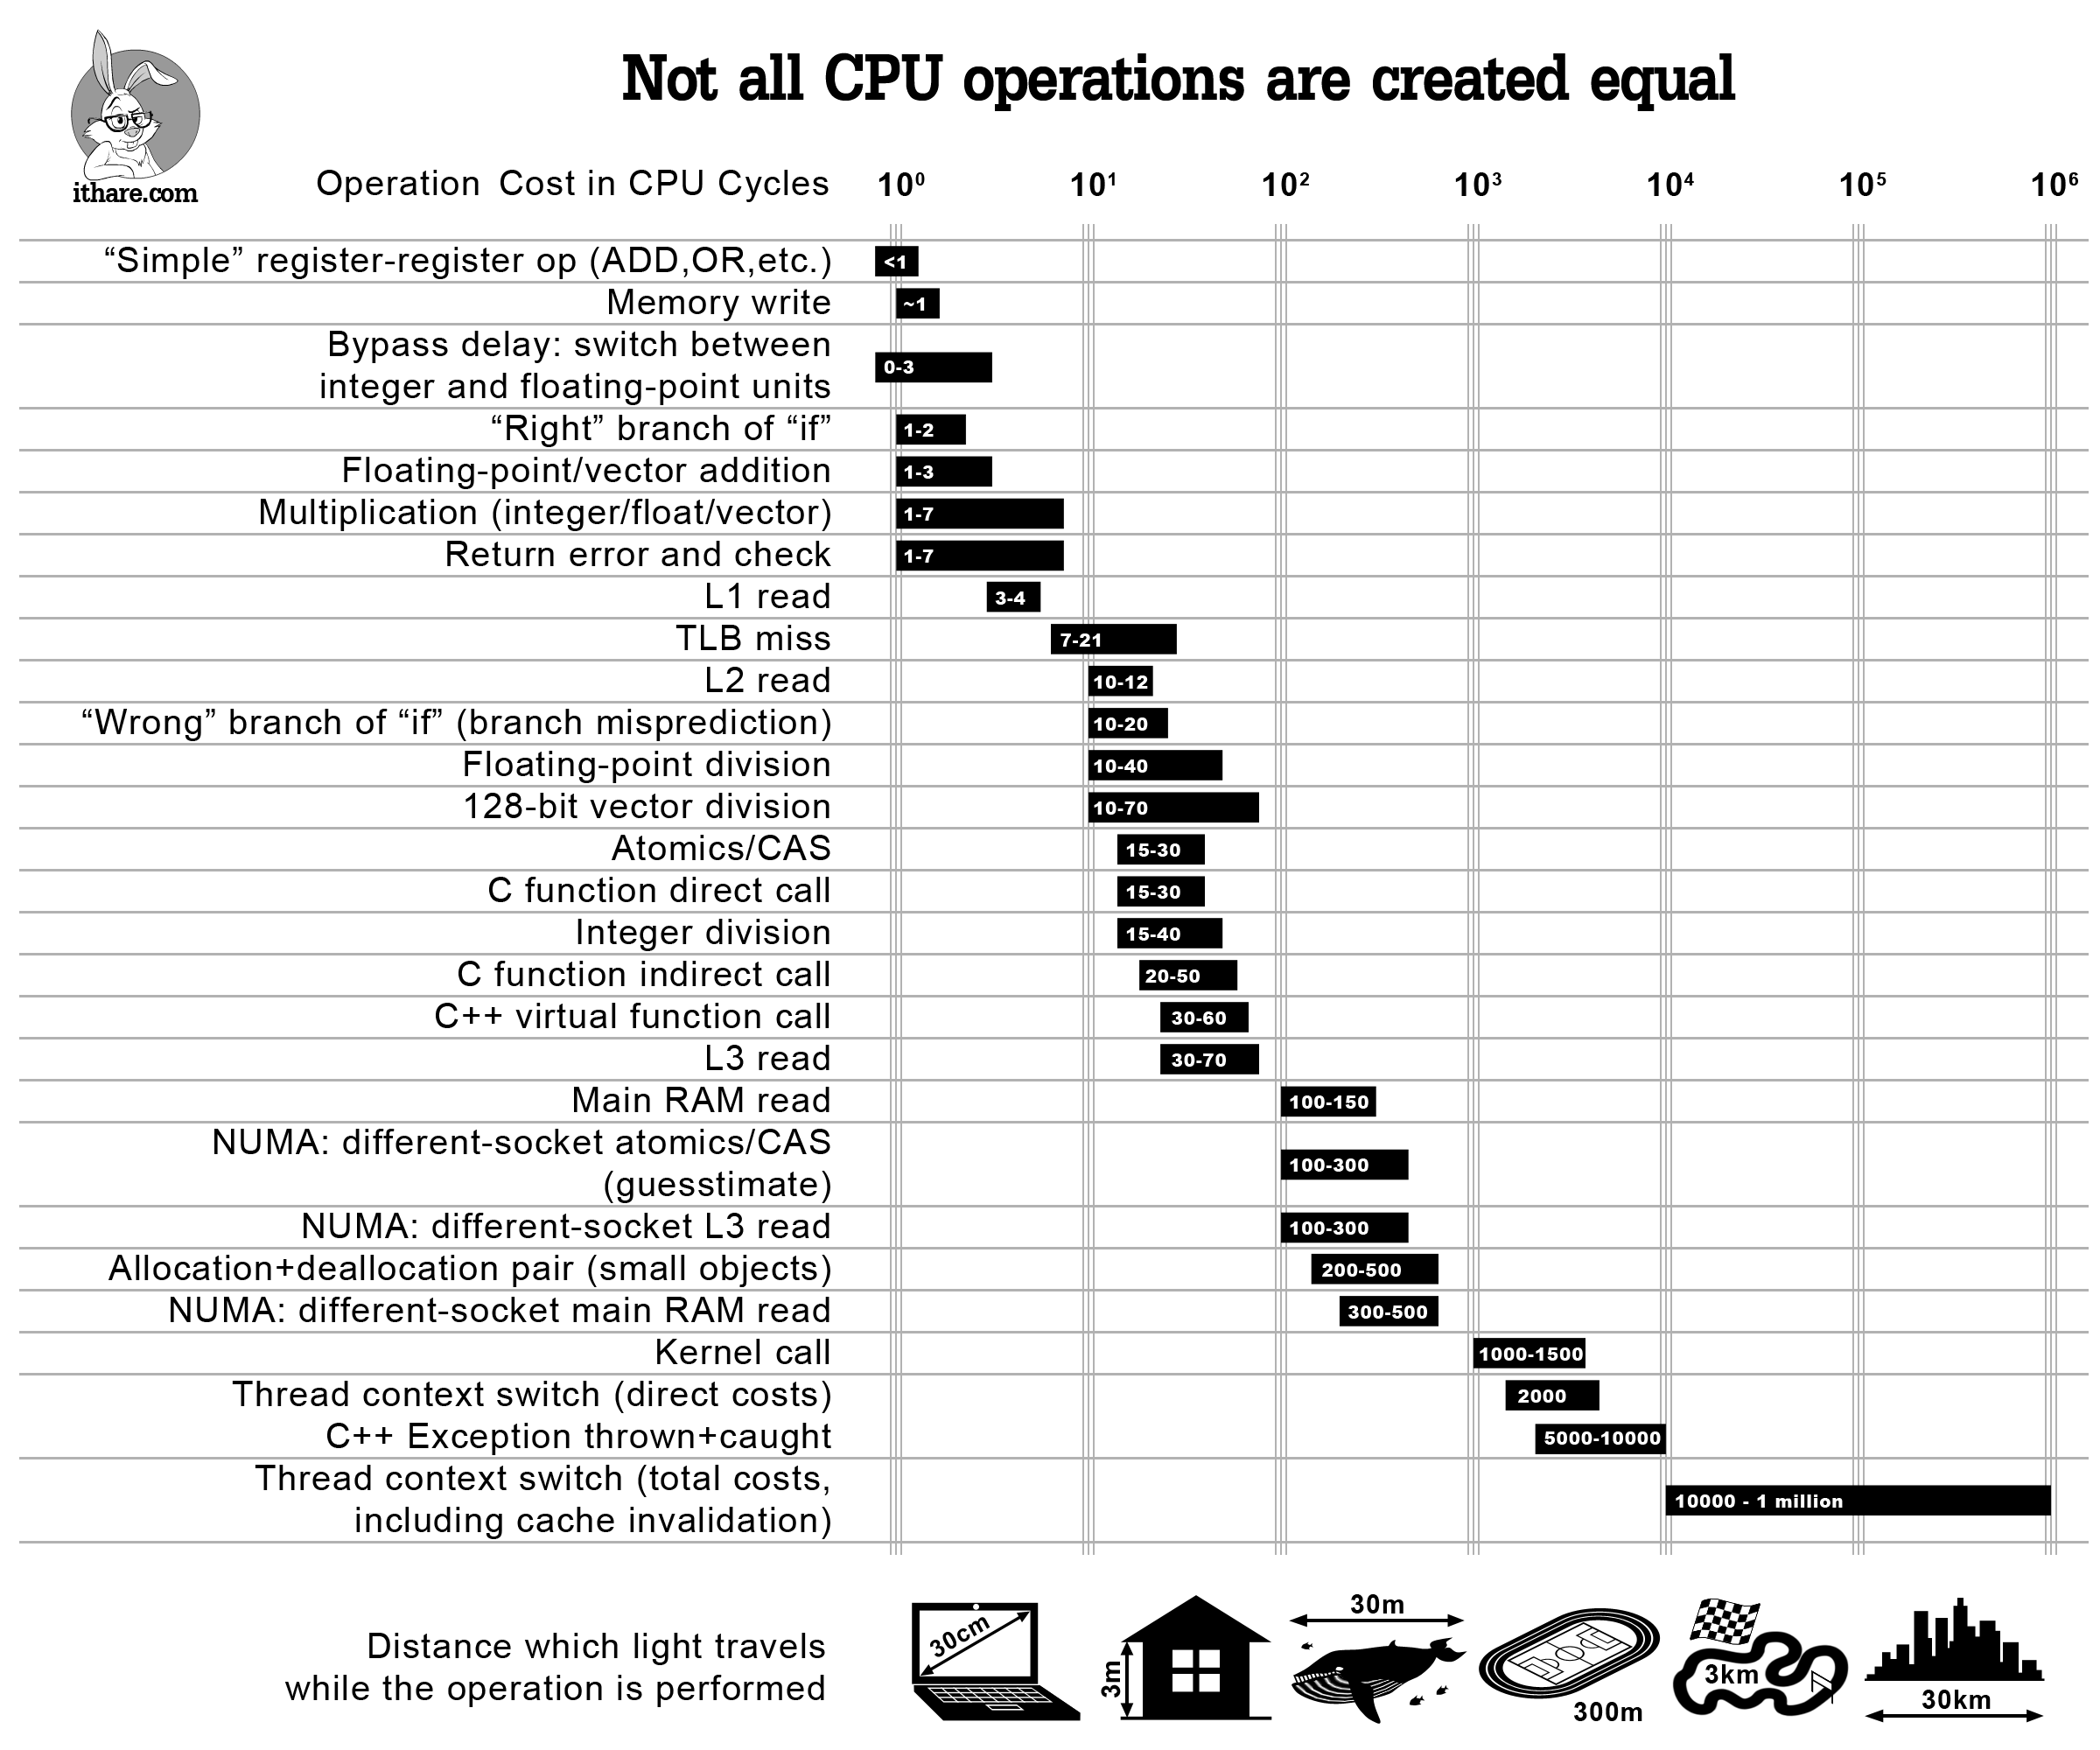
\includegraphics[width=0.9\textwidth]{part101_infographics_v08}
\caption{Operation Costs in CPU Clock Cycles\cite{archcost}}
\end{figure}

For instance, for an x86 CPU, the associated rComplexity class would be
$ O_{1}(c_{noConflict} * n) $, where $c_{noConflict}$ is a constant corresponding to the no. of cycles required to perform the operations inner the for-loop.

For the pseudocode:
\begin{algorithmic}[1]
	\For {i=1..row-1}
		\If {currentMatrix[i][column] = 1}
			\State \Return FALSE
		\EndIf
	\EndFor
\end{algorithmic}
In a broad manner, we can estimate that the cost for the inner snippet is $c_{computeOffset} + c_{readMemory} + c_{check=1}$, where in order to compute offset, we need to perform $i * ROWS + column$, so
$ c_{computeOffset} = O_{1}(c_{addition} + c_{multiplication} + 3 * c_{readMemory})$.

Looking in a x86 Cycle cost table for operation, we can estimate the primitives $c_{addition} = O_{1}(4)$ and $c_{multiplication} = O_{1}(4)$. For memory access, the time varies, on reasons based on cache mechanics, prefetch and other runtime mechanism for improvement in speed of read operations. A satisfying margin would be $c_{readMemory} = O_{1}(100)$. 

Suppose for a complete check and jump in code $c_{check=1} = 10$.

Therefore, for the inner snippet using the abose estimations, the rComplexity would be $O_{1}(4 * 100 + 4 + 4 + 10) = O_{1}(418)$. Now, the whole snippet will have the complexity $O_{1}((418 + c_{for\_checks}) \cdot n)$, where  $c_{for\_checks} = c_{check=row} + c_{addition}$ is the associated cost for incrementing the index and other checks. 

Thus, the rComplexity of the snippet is $O_{1}((418 + 14) \cdot n) = O_{1}(432 \cdot n)$ using the abose estimations.

 
For an exact value, we need to check the associated generated assembly code for the architecture (example x86-32bit):
\begin{verbatim}
f:
        push    ebp
        mov     ebp, esp
        sub     esp, 16
        mov     DWORD PTR [ebp-4], 0
        jmp     .L2
.L5:
        mov     eax, DWORD PTR [ebp-4]
        imul    edx, eax, 400
        mov     eax, DWORD PTR [ebp+16]
        add     edx, eax
        mov     eax, DWORD PTR [ebp+12]
        mov     eax, DWORD PTR [edx+eax*4]
        cmp     eax, 1
        je      .L6
        add     DWORD PTR [ebp-4], 1
.L2:
        mov     eax, DWORD PTR [ebp-4]
        cmp     eax, DWORD PTR [ebp+8]
        jl      .L5
        jmp     .L1
.L6:
        nop
.L1:
        leave
        ret  
\end{verbatim}


The inner loop calculus are provided inner $.L5$ label. Having this code and the x86 cycles/instructions table, we can calculate the ideal rComplexity $\Theta_{1}(n \cdot (c_{.L2} + c_{.L5}))$. 

Also, $c_{.L2} = c_{mov} + c_{cmp} + c_{li}$ and $c_{.L5} = c_{mov} + c_{imul} + c_{mov} +  c_{add} + c_{mov} + c_{mov} + c_{cmp} + c_{je} + c_{add} $. 

Using reflexivity, we conclude the rComplexity of the snippet 1 is \[f_{snippet_{1}} =  \Theta_{1}(n \cdot ( 5 * c_{mov} + c_{imul} + 2 * c_{add} +2 *  c_{cmp} + c_{je} + c_{li}))\]

Having this snippet's associated complexity calculated, we can proceed to calculate the other independent for-loops in the noConflict function:
\begin{algorithmic}[1]
	\For {j=column..n}
	\If {currentMatrix[i][j] = 1}
			\State \Return FALSE
		\EndIf
	\If {$i \leq 0$}
		\State break
	\EndIf
	\State $i \gets i-1$	
	\EndFor
\end{algorithmic}
We will associate the complexity function of this snippet with $f_{snippet_{2}}$. Similarly, for the snippet:

\begin{algorithmic}[1]
	\For {j=column..0 : increment -1}
	\If {currentMatrix[i][j] = 1}
			\State \Return FALSE
		\EndIf
	\If {$i \leq 0$}
		\State break
	\EndIf
	\State $i \gets i-1$	
	\EndFor
\end{algorithmic}
a complexity function will be obtained described by $f_{snippet_{3}}$.

Using addition properties, the complexity function for the procedute noConflict will be $f_{snippet_{1}} + f_{snippet_{2}} + f_{snippet_{3}} = O_{1}(c_{noConflict} \cdot n)$., where $c_{noConflict} \cdot n$ is the architecture-dependant constant.

 For instance, for x86, we can approximate $c_{noConflict \cdot n} = 432 * 3 = 1296$ and $f_{snippet_{1}} + f_{snippet_{2}} + f_{snippet_{3}} = O_{1}(1296 \cdot n) $.



Going deeper tracing the flow, we can evaluate the complexity of QueenProblem procedure by checking all elements involved in the procedure.
 \[QueenProblem(n) = O_{1}(recursiveCall) + O_{1}(noConflict) + O_{1}(overhead) + O_{1}(basecase) \]
Therefore:
 \[\begin{cases} QueenProblem(n) = n \cdot QueenProblem(n-1) +  O_{1}(1296 \cdot n) (c_{overheadFor} + c_{setBitsMatrix}) \cdot O_{1}(n) \\ QueenProblem_{1}(1)=O_{1}(c_{printMatrix}) \end{cases}\]
 where $O_{1}(1296 \cdot n)$ is the rComplexity for the noConflict check.
 
Using the previous estimation, we assume $c_{overheadFor} = 14$ and $c_{setBitsMatrix} = 108$. Thus, the recurrent equation looks as follows: 
\[QueenProblem(n) = n \cdot QueenProblem(n-1) +  O_{1}(1418 \cdot n) \]

For the base case, we need to find the complexity of printMatrix method.
\[ \begin{cases} QueenProblem(1)=O_{1}(n^{2} \cdot  (c_{computeOffset} + c_{readMatrixElement})) \\ QueenProblem(1)=O_{1}(n^{2} \cdot  408) \end{cases}\]

For simplicity, we can rewrite:
\[ \begin{cases} QueenProblem(n) = n \cdot QueenProblem(n-1) +  1418 \cdot O_{1}(n) \\ QueenProblem(1)= 408 \cdot O_{1}(n^{2}) \end{cases}\]

We can model the system as an recurrence equation:
\[ g(n) = n \cdot  g(n-1) + 1418 \cdot  n; g(0) = 408 \cdot  n^{2} \]
with the solution:
\[ 408 \cdot n^{3} \cdot \Gamma(n) + 1418 \cdot e \cdot  n \cdot \Gamma(n, 1)\]
where $\Gamma$ represents the \textit{gamma function} that satisfies: \[ \Gamma \left( x \right) = \int\limits_0^\infty {s^{x - 1} e^{ - s} ds} \] and $ \Gamma(n,x)$ represents the \textit{incomplete gamma function} that satisfies: \[ \Gamma \left(x, n \right) = \int\limits_n^\infty {s^{x - 1} e^{ - s} ds}\]

The solution of this recurrence equation in rComplexity calculus (with $n \in \mathbb{N}$) is:
\[ QueenProblem(n) = O_{1}(408 \cdot n^{2} \cdot n!) +  O_{1}(1418 \cdot n \cdot n!) \]
Using the $O_{1}$ addition properties, we conclude:
\[ QueenProblem(n) = O_{1}(408 \cdot n^{2} \cdot n!) \]

\begin{remark}
The rComplexity function associated with the algorithm $(408 \cdot n^{2} \cdot n!)$ is from the same tradition complexity class as calculated before $ O(n^2\cdot n!)$.
\end{remark}


\section{Automatic estimation of rComplexity}
This section aims to present a solution for automation for calculating an approximate of the associated rComplexity class for any given algorithm. The prerequisites for this method implies a technique for obtaining relevant metric-specific details for diversified input dimensions. For instance, if time is the monitored metric, there must exist a collection of pertinent data linking the correspondence between input size and the total execution time for the designated input size.

\subsection{Estimation for algorithms with known Bachmann–Landau Complexity}
Reckoning an associated rComplexity class ($f$) for an algorithm with established Bachmann–Landau Complexity ($g$) consists in the process of tailoring an suitable constant $c$, such that $f \approx \Theta_{1}(c \cdot g)$ or in Big-O calculus, $f \leq  \mathbb{O}_{1} (c \cdot g)$. The approach presented below is a particularized version of linear regression, which attempts to model the relationship between various variables by fitting a linear equation to observed data. Even if the model generally follows the classical pattern of a Machine Learning Process (training, predicting, etc.), where a training example consists of a pair ($inputSize$, $metricValue$).

A trick is used to adjust the entry values if the Bachmann–Landau relationship between the $inputSize$ and the metric is known. In order to adjust the learning set to a more knowledgeable set, we can extract new features and replace all the ($inputSize$, $metricValue$) pairs with ($g(inputSize)$, $metricValue$), where $g$ is the known Bachmann–Landau Complexity function converted into Normal form.


The importance of this trick can be emphasized comparing the classical linear regression model with various learning datasets. For the matrix multiplication problem, a naive algorithm (with Bachmann–Landau Complexity $\mathbb{O}(n^{3})$) has been implemented. After testing, the algorithm has been deployed and executed matrix multiplications for various sizes of the matrixes. The execution has been audited and the results have been summarized in the following table, which represents the correspondance between matrix dimension and running time:

\begin{table}[H]
\begin{center}
\scalebox{0.6}{
\begin{tabular}{|l|l|l|l|l|l|l|l|l|l|l|l|}
\hline
\begin{tabular}[c]{@{}l@{}}input\\ Size\end{tabular} & Time $(s)$     & \begin{tabular}[c]{@{}l@{}}input\\ Size\end{tabular} & Time $(s)$  & \begin{tabular}[c]{@{}l@{}}input\\ Size\end{tabular} & Time $(s)$  & \begin{tabular}[c]{@{}l@{}}input\\ Size\end{tabular} & Time $(s)$  & \begin{tabular}[c]{@{}l@{}}input\\ Size\end{tabular} & Time $(s)$   & \begin{tabular}[c]{@{}l@{}}input\\ Size\end{tabular} & Time $(s)$   \\ \hline
16                                                   & 0.000018 & 1024                                                 & 8.52   & 2112                                                 & 123.73 & 3200                                                 & 462.71 & 4288                                                 & 999.25  & 5376                                                 & 1647.23 \\ \hline
32                                                   & 0.000339 & 1088                                                 & 10.96  & 2176                                                 & 135.21 & 3264                                                 & 358.01 & 4352                                                 & 864.15  & 5440                                                 & 1929.46 \\ \hline
48                                                   & 0.001123 & 1152                                                 & 13.76  & 2240                                                 & 149.43 & 3328                                                 & 540.64 & 4416                                                 & 987.71  & 5504                                                 & 1693.75 \\ \hline
64                                                   & 0.001468 & 1216                                                 & 18.03  & 2304                                                 & 148.82 & 3392                                                 & 446.29 & 4480                                                 & 1095.01 & 5568                                                 & 1986.99 \\ \hline
128                                                  & 0.015482 & 1280                                                 & 21.55  & 2368                                                 & 180.07 & 3456                                                 & 592.91 & 4544                                                 & 1126.39 & 5632                                                 & 2002.14 \\ \hline
256                                                  & 0.084991 & 1344                                                 & 25.59  & 2432                                                 & 117.83 & 3520                                                 & 480.98 & 4608                                                 & 1147.28 & 5696                                                 & 2013.22 \\ \hline
320                                                  & 0.172411 & 1408                                                 & 30.66  & 2496                                                 & 213.51 & 3584                                                 & 621.36 & 4672                                                 & 1280.23 & 5760                                                 & 2066.87 \\ \hline
384                                                  & 0.296398 & 1472                                                 & 28.27  & 2560                                                 & 236.41 & 3648                                                 & 582.46 & 4736                                                 & 1228.73 & 5824                                                 & 2029.52 \\ \hline
448                                                  & 0.535461 & 1536                                                 & 41.91  & 2624                                                 & 255.39 & 3712                                                 & 628.36 & 4800                                                 & 1222.14 & 5888                                                 & 2236.73 \\ \hline
512                                                  & 0.764842 & 1600                                                 & 48.90  & 2688                                                 & 275.05 & 3776                                                 & 650.76 & 4864                                                 & 1256.73 & 5952                                                 & 2503.13 \\ \hline
576                                                  & 1.308485 & 1664                                                 & 56.34  & 2752                                                 & 167.51 & 3840                                                 & 651.43 & 4928                                                 & 1290.35 & 6016                                                 & 2317.91 \\ \hline
640                                                  & 1.803608 & 1728                                                 & 70.47  & 2816                                                 & 268.64 & 3904                                                 & 626.79 & 4992                                                 & 1488.43 & 6080                                                 & 2395.12 \\ \hline
704                                                  & 2.516613 & 1792                                                 & 71.02  & 2880                                                 & 296.00 & 3968                                                 & 659.29 & 5056                                                 & 1432.41 & 6144                                                 & 2718.02 \\ \hline
768                                                  & 3.334002 & 1856                                                 & 84.41  & 2944                                                 & 304.91 & 4032                                                 & 915.86 & 5120                                                 & 1093.62 &                                                      &         \\ \hline
832                                                  & 4.315076 & 1920                                                 & 67.05  & 3008                                                 & 300.06 & 4096                                                 & 769.01 & 5184                                                 & 1649.00 &                                                      &         \\ \hline
896                                                  & 5.571474 & 1984                                                 & 99.74  & 3072                                                 & 228.34 & 4160                                                 & 864.89 & 5248                                                 & 1729.42 &                                                      &         \\ \hline
960                                                  & 7.076612 & 2048                                                 & 110.90 & 3136                                                 & 446.72 & 4224                                                 & 789.13 & 5312                                                 & 1743.26 &                                                      &         \\ \hline
\end{tabular}
}
\end{center}
\caption{Reported timings for different input size for a naive matrix multiplication algorithm in $\mathbb{O}(n^{3})$. Results have been obtained on an i5 3.2GHz, x86\_64 Architecture with L1d cache: 32K, L1i cache: 32K, L2 cache: 256K, L3 cache:  6144K}
\end{table}

Training a linear regression model on this dataset would result in model with a linear equation to observed data, similar with the one below(a). Translation of the dataset can enhance fitting results for the regression. Examples for ($inputSize$, $metricValue$) $ \Rightarrow $ ($inputSize^{n}$, $metricValue$) are presented in (b) $n = 2$, (c) $n = 3$ and (d) $n = 4$.


\begin{table}[H]
\begin{center}
\scalebox{0.6}{
\begin{tabular}{|l|l|l|l|l|l|l|l|l|l|l|l|}
\hline
\begin{tabular}[c]{@{}l@{}}input\\ Size$^3$ \end{tabular} & Time $(s)$     & \begin{tabular}[c]{@{}l@{}}input\\ Size$^3$\end{tabular} & Time $(s)$  & \begin{tabular}[c]{@{}l@{}}input\\ Size$^3$\end{tabular} & Time $(s)$  & \begin{tabular}[c]{@{}l@{}}input\\ Size$^3$\end{tabular} & Time $(s)$  & \begin{tabular}[c]{@{}l@{}}input\\ Size$^3$\end{tabular} & Time $(s)$   & \begin{tabular}[c]{@{}l@{}}input\\ Size$^3$\end{tabular} & Time $(s)$   \\ \hline
4.10E+03  & 0.000018 & 1.07E+09  & 8.52   & 9.42E+09  & 123.73 & 3.28E+10  & 462.71 & 7.88E+10  & 999.25  & 1.55E+11  & 1647.23 \\ \hline
3.28E+04  & 0.000339 & 1.29E+09  & 10.96  & 1.03E+10  & 135.21 & 3.48E+10  & 358.01 & 8.24E+10  & 864.15  & 1.61E+11  & 1929.46 \\ \hline
1.11E+05  & 0.001123 & 1.53E+09  & 13.76  & 1.12E+10  & 149.43 & 3.69E+10  & 540.64 & 8.61E+10  & 987.71  & 1.67E+11  & 1693.75 \\ \hline
2.62E+05  & 0.001468 & 1.80E+09  & 18.03  & 1.22E+10  & 148.82 & 3.90E+10  & 446.29 & 8.99E+10  & 1095.01 & 1.73E+11  & 1986.99 \\ \hline
2.10E+06  & 0.015482 & 2.10E+09  & 21.55  & 1.33E+10  & 180.07 & 4.13E+10  & 592.91 & 9.38E+10  & 1126.39 & 1.79E+11  & 2002.14 \\ \hline
1.68E+07  & 0.084991 & 2.43E+09  & 25.59  & 1.44E+10  & 117.83 & 4.36E+10  & 480.98 & 9.78E+10  & 1147.28 & 1.85E+11  & 2013.22 \\ \hline
3.28E+07  & 0.172411 & 2.79E+09  & 30.66  & 1.56E+10  & 213.51 & 4.60E+10  & 621.36 & 1.02E+11  & 1280.23 & 1.91E+11  & 2066.87 \\ \hline
5.66E+07  & 0.296398 & 3.19E+09  & 28.27  & 1.68E+10  & 236.41 & 4.85E+10  & 582.46 & 1.06E+11  & 1228.73 & 1.98E+11  & 2029.52 \\ \hline
8.99E+07  & 0.535461 & 3.62E+09  & 41.91  & 1.81E+10  & 255.39 & 5.11E+10  & 628.36 & 1.11E+11  & 1222.14 & 2.04E+11  & 2236.73 \\ \hline
1.34E+08  & 0.764842 & 4.10E+09  & 48.90  & 1.94E+10  & 275.05 & 5.38E+10  & 650.76 & 1.15E+11  & 1256.73 & 2.11E+11  & 2503.13 \\ \hline
1.91E+08  & 1.308485 & 4.61E+09  & 56.34  & 2.08E+10  & 167.51 & 5.66E+10  & 651.43 & 1.20E+11  & 1290.35 & 2.18E+11  & 2317.91 \\ \hline
2.62E+08  & 1.803608 & 5.16E+09  & 70.47  & 2.23E+10  & 268.64 & 5.95E+10  & 626.79 & 1.24E+11  & 1488.43 & 2.25E+11  & 2395.12 \\ \hline
3.49E+08  & 2.516613 & 5.75E+09  & 71.02  & 2.39E+10  & 296.00 & 6.25E+10  & 659.29 & 1.29E+11  & 1432.41 & 2.32E+11  & 2718.02 \\ \hline
4.53E+08  & 3.334002 & 6.39E+09  & 84.41  & 2.55E+10  & 304.91 & 6.55E+10  & 915.86 & 1.34E+11  & 1093.62 &           &         \\ \hline
5.76E+08  & 4.315076 & 7.08E+09  & 67.05  & 2.72E+10  & 300.06 & 6.87E+10  & 769.01 & 1.39E+11  & 1649.00 &           &         \\ \hline
7.19E+08  & 5.571474 & 7.81E+09  & 99.74  & 2.90E+10  & 228.34 & 7.20E+10  & 864.89 & 1.45E+11  & 1729.42 &           &         \\ \hline
8.85E+08  & 7.076612 & 8.59E+09  & 110.90 & 3.08E+10  & 446.72 & 7.54E+10  & 789.13 & 1.50E+11  & 1743.26 &           &         \\ \hline
\end{tabular}
}
\end{center}
\caption{Training data for the linear regression model after mapping ($inputSize$, $metricValue$) pairs with ($inputSize^3$, $metricValue$)}
\end{table}

\begin{figure}[H]
\makebox[\textwidth][c]{\parbox{1.2\textwidth}{%
  \begin{subfigure}{.6\textwidth}
      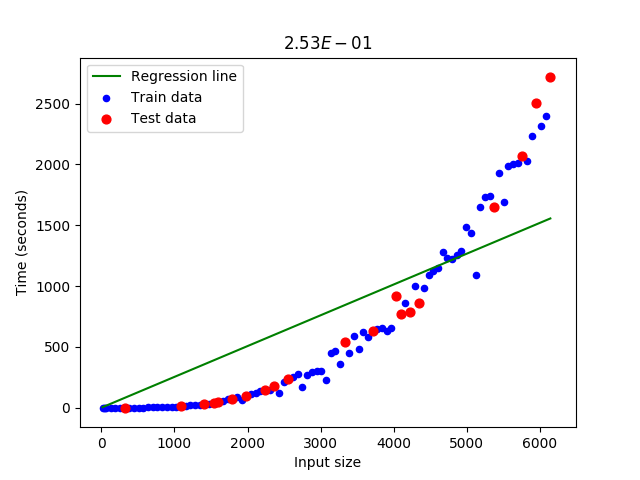
\includegraphics[width=\linewidth]{mm521_1.png}
      \caption{Linear Regression Model trained with initial features $g(n) = n^1 $}
  \end{subfigure}%
  \begin{subfigure}{.6\textwidth}
      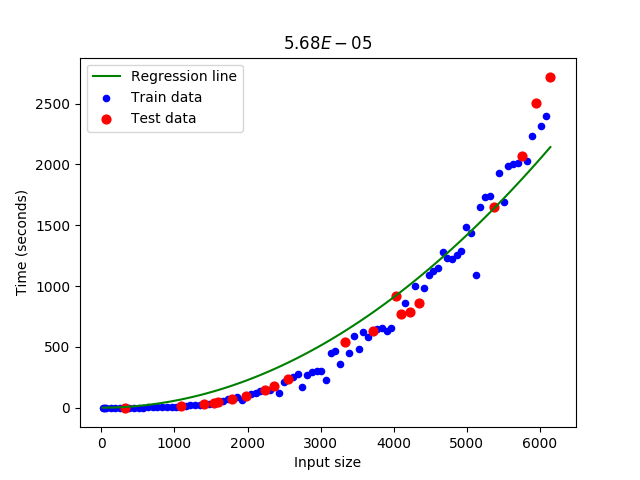
\includegraphics[width=\linewidth]{mm521_2.png}
      \caption{Linear Regression Model trained with new features obtained using $g(n) = n^2 $}
  \end{subfigure}
  \begin{subfigure}{.6\textwidth}
      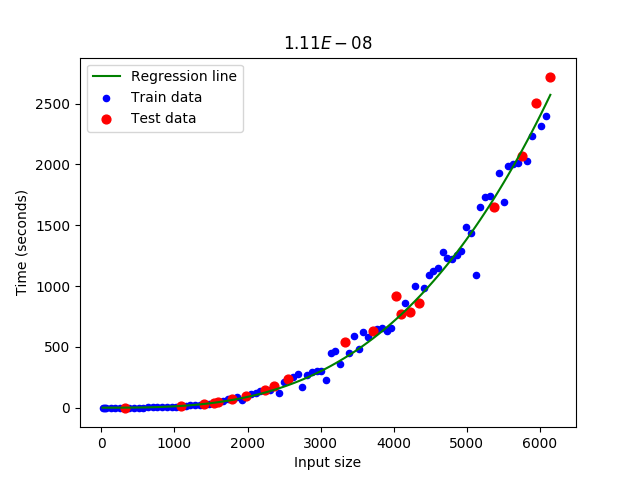
\includegraphics[width=\linewidth]{mm521_3.png}
      \caption{Linear Regression Model trained with new features obtained using $g(n) = n^3$}
  \end{subfigure}%
  \begin{subfigure}{.6\textwidth}
      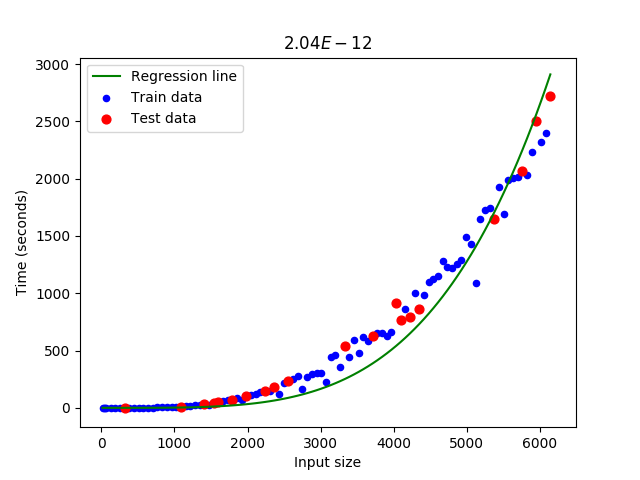
\includegraphics[width=\linewidth]{mm521_4.png}
      \caption{Linear Regression Model trained with new features obtained using $g(n) = n^4$}
  \end{subfigure}
}}
\caption{Various prediction boundaries based on accommodated training dataset using multiple relations $g$. Training data are obtained for different input size for a naive matrix multiplication algorithm in $\mathbb{O}(n^{3})$}
\end{figure}

As an intuition, the natural fit was obtained when using $g(n) = n^3$ with consideration to generalization. If we choose bigger degree polynomial transformations, we may obtain better results on this datasets, but the models are becoming subject to overfit. The subject of Matrix multiplication is furthered discussed in a distinct section. 


\subsection{Estimation for algorithms with unknown Bachmann–Landau Complexity}
Estimation for algorithms with unknown Bachmann–Landau Complexity becomes a lot more difficult as there are numerous possible candidates for a matching complexity function. 

A general polynomial Performance model normal form is presented in Chapter 2.1 Automatic Empirical Performance Modeling of Parallel Programs \cite{calotoiu2018automatic}. An enhance model for complexity functions should contain also an exponential behavior, which is often seen as a synergy between NP-Hard problems. Thus, we propose the following general expression:

\[ f(n) =\sum\limits_{t=1}^{y}  \sum\limits_{k=1}^{x} c_{k} \cdot n^{p_{k}} \cdot log_{l_{k}}^{j_{k}}(n) \cdot e_{t}^{n} \cdot  \Gamma(n)^{g_{k}} \]
This representation is, of course, not exhaustive, but it works in most practical schemes. An intuitive motivation is a consequence of how most computer algorithms are designed. \cite{calotoiu2018automatic}



\section{Matrix multiplication}
In this section, we aim to provide an example of estimation for matrix multiplication algorithms with known Bachmann–Landau Complexity.

Matrix multiplication plays very important role in many scientific disciplines because of fact that it is considered as the main tool for many other computations in different areas, like those in seismic analysis, different simulations (like galactic simulations), aerodynamic computations, signal and images processing. \cite{4588528}


\begin{figure}[H]
\centering
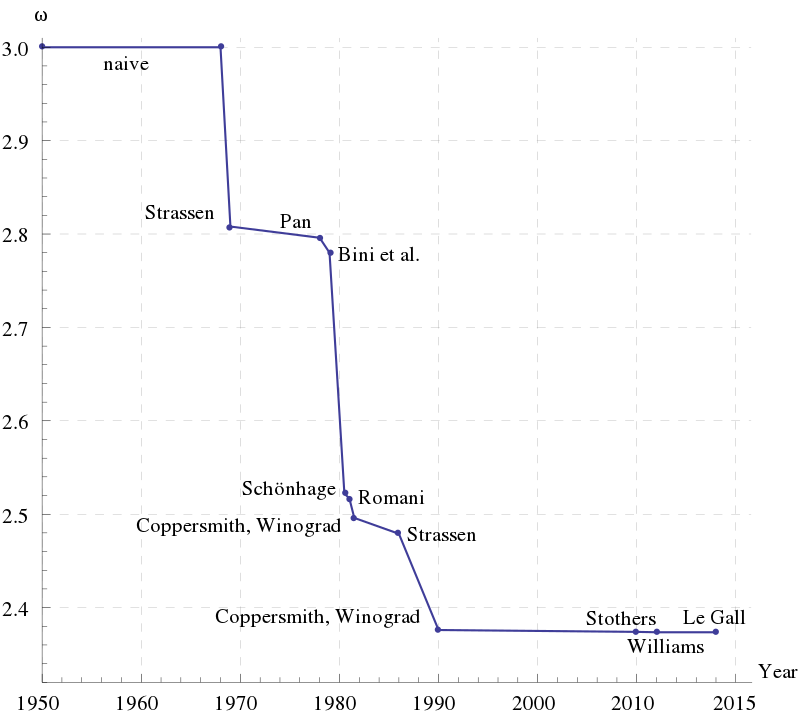
\includegraphics[width=0.6\textwidth]{matrixC}
\caption{Before 1969, all known matrix multiplication algorithm were in $O(n^3)$. After Volker Strassen first published this algorithm and proved that the naive algorithm wasn't optimal, various attempts to narrow down the exponent $\omega$ appeared. One big breakthrough was brought by Coppersmith–Winograd algorithm, with complexity $O(n^{2.375})$. }
\end{figure}

We analyzed various naive matrix multiplication algorithms $O(n^3)$ with memory-access improvements (cache-locality of loops, Blocked Matrix Multiplication) and an efficient implementation of Strassen algorithm.

\begin{figure}[H]
\centering
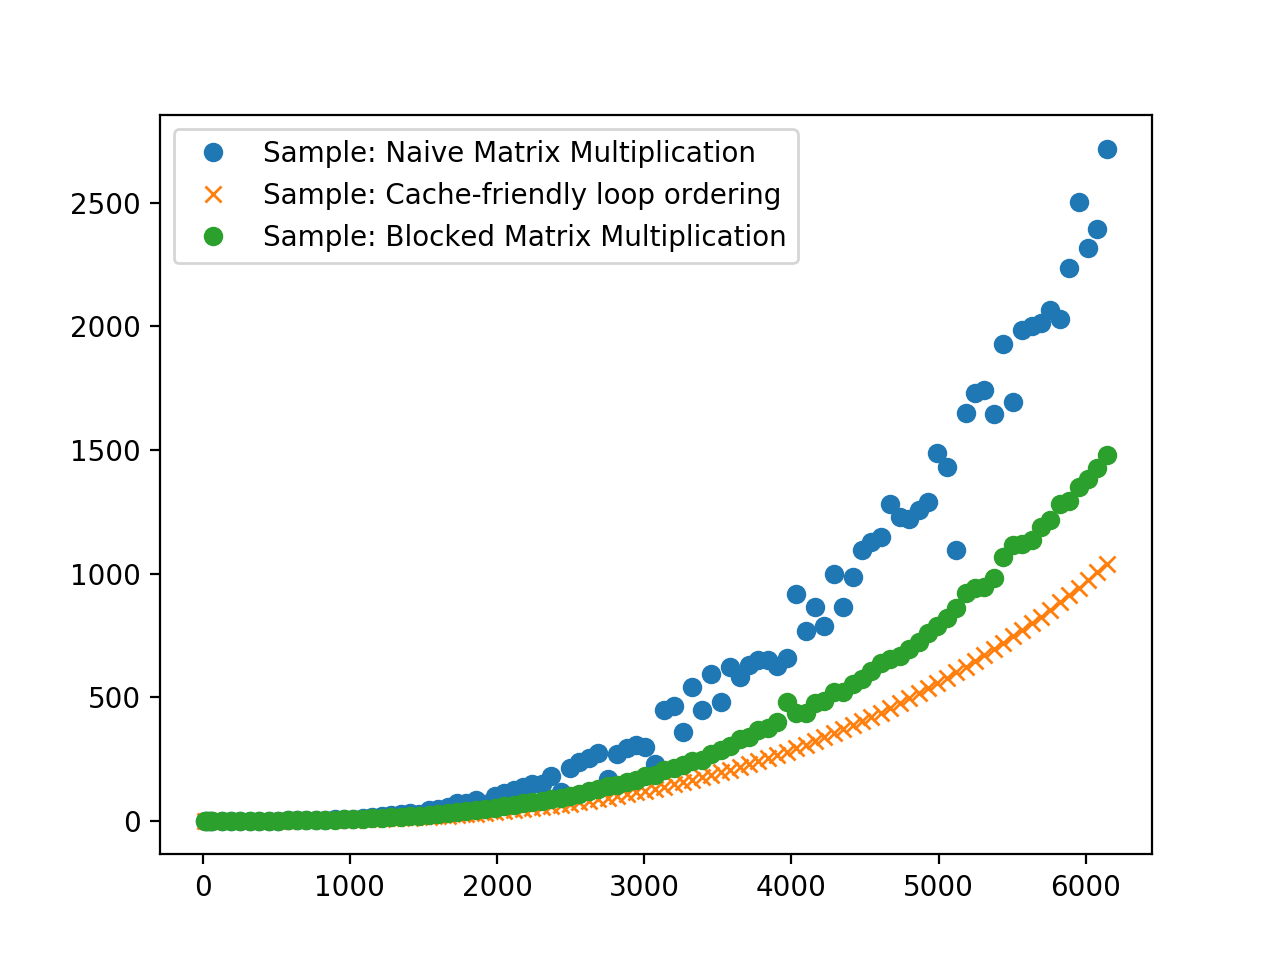
\includegraphics[width=0.7\textwidth]{matrixn3all}
\caption{The results above have been reported on an i5 3.2GHz, x86\_64 Architecture with L1d cache: 32K, L1i cache: 32K, L2 cache: 256K, L3 cache:  6144K. We do not postulate that the methods above cannot be enhanced
 or the efficiency of the optimizations are in a specific order. We aim to provide various estimation for these implementations of matrix multiplication algorithms with known $O(n^3)$ Complexity. Please remark the natural distribution of the two cache-friendly algorithms presented on larger datasets vs the naive algorithm, susceptible to outliers. }
\end{figure}


Using the method described in estimating section, we can tailor an architecture-specific complexity function $ f(n)  = c \cdot n^3$.

\begin{figure}[H]
\centering
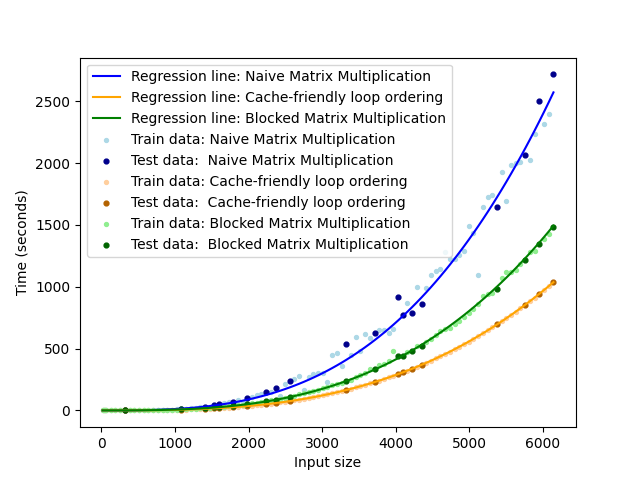
\includegraphics[width=0.7\textwidth]{mmn3023}
\caption{TODO}
\end{figure}

After training the regression models for each algorithm, we obtained the coefficients $c$, that defines the complexity function $f(n)  = c \cdot n^3$.
\begin{table}[H]
\centering
\begin{tabular}{|
>{\columncolor[HTML]{FFCCC9}}l |
>{\columncolor[HTML]{32CB00}}l |}
\hline
\cellcolor[HTML]{C0C0C0}\textit{\textbf{Algorithm}} & \cellcolor[HTML]{C0C0C0}{\color[HTML]{000000} \textit{\textbf{\begin{tabular}[c]{@{}l@{}}Complexity\\ Function\end{tabular}}}} \\ \hline
\textbf{Naive Matrix Multiplication}                & {$ 1.109 \cdot 10^{-8} \cdot n^3 $}                                                                                      \\ \hline
\textbf{Cache-friendly loop ordering}               & {$4.472e \cdot 10^{-9} \cdot n^3 $ }                                                                                      \\ \hline
\textbf{Blocked Matrix Multiplication}              & {$6.441e \cdot 10^{-9} \cdot n^3 $ }                                                                                      \\ \hline
\end{tabular}
\caption{The regression model was evaluating using the above metrics: Root Mean Square Error (RMSE) and $R^2$ (coefficient of determination) regression score function}
\end{table}


Furthermore, the model was evaluated adopting classical regression evaluation metrics, independently settled on training and testing data.
\begin{table}[H]
\begin{tabular}{|
>{\columncolor[HTML]{FFCCC9}}l |
>{\columncolor[HTML]{32CB00}}l |
>{\columncolor[HTML]{FFFFFF}}l |
>{\columncolor[HTML]{FFFFFF}}l |
>{\columncolor[HTML]{FFFFFF}}l |
>{\columncolor[HTML]{FFFFFF}}l |}
\hline
\cellcolor[HTML]{C0C0C0}\textit{\textbf{Algorithm}} & \cellcolor[HTML]{C0C0C0}{\color[HTML]{000000} \textit{\textbf{c}}} & \cellcolor[HTML]{C0C0C0}\textit{\begin{tabular}[c]{@{}l@{}}{[}Training{]}\\ RMSQ\end{tabular}} & \cellcolor[HTML]{C0C0C0}\textit{\begin{tabular}[c]{@{}l@{}}{[}Training{]}\\ R2 score\end{tabular}} & \cellcolor[HTML]{C0C0C0}\begin{tabular}[c]{@{}l@{}}{[}Test{]}\\ RMSQ:\end{tabular} & \cellcolor[HTML]{C0C0C0}\textit{\begin{tabular}[c]{@{}l@{}}{[}Test{]}\\ R2 score\end{tabular}} \\ \hline
\textbf{Naive Matrix Multiplication}                & {\color[HTML]{000000} \textit{1.109e-08}}                          & {\color[HTML]{000000} 5740.95}                                                                     & 0.9886                                                                                                 & 6136.10                                                                                & {\color[HTML]{000000} 0.9912}                                                                      \\ \hline
\textbf{Cache-friendly loop ordering}               & {\color[HTML]{000000} \textit{4.472e-09}}                          & {\color[HTML]{000000} 0.2517}                                                                      & 0.9999969                                                                                              & 0.2917                                                                                 & {\color[HTML]{000000} 0.999997}                                                                    \\ \hline
\textbf{Blocked Matrix Multiplication}              & {\color[HTML]{000000} \textit{6.441e-09}}                          & 185.70                                                                                             & 0.9989                                                                                                 & 63.64                                                                                  & {\color[HTML]{000000} 0.99971}                                                                     \\ \hline

\end{tabular}
\caption{The regression model was evaluated using the above metrics: Root Mean Square Error (RMSE) and $R^2$ (coefficient of determination) regression score function}
\end{table}
\chapter{The web of complexities}

\section{Modern means of computing}
\textbf{The world of computing} has been \textit{vastly} changed by \textit{modern means of inter-components communication}, allowing computing systems to \textit{geographically} extend at an affordable overhead. This allowed the emergence of new software services as well as \textbf{new means of programming}. 

Undoubtedly, \textit{the internet} has become a massive source of power and with this new technology the information is able to spread really quickly around the world.

While there are many notable achievements in software services that were created over networks, \textit{including e-commerce platforms, social media services or e-Gov apps}, the focus of this chapter is to embrace the new paradigm of \textbf{distributed computing and web development} on \textbf{complexity calculus} and \textit{present means of computing} an estimated complexity for complex applications that require new features such as mechanisms for \textit{networking handling} which have not been analyzed yet.

\section{HTTP requests and algorithm complexity}

There are numerous way of inter-system communication, provided by powerful protocols. Undoubtable, the most used communication protocol between software systems is \textbf{HTTP} (Hypertext Transfer Protocol), an application-level protocol for distributed, collaborative, hypermedia information systems. HTTP operates as a \textit{request - response protocol} in the \textit{client - server  model}.

The \textit{scenario of development} when the client sends a request to the server and the server send an associated response is frequently encountered in \textit{web applications development}. We will analyze how to integrate this \textit{overhead} in the complexity model presented.

Consider the following \textit{scenario}: The results of this paper appears to be interesting and you may want to re-use them and further analyze them. You built your custom computer program and you want to acquire all practical results provided so far. Note that the development might still be in progress, so you would like that every time you run the software, an up-to-date version of all results should be available. Luckily, these can be achieved via HTTP-requests, as all of the results are stored publicly on GitHub. Therefore, you can use GitHub Developer API, to view the latest published full release for the repository.

\begin{verbatim}
GET /repos/:owner/:repo/releases/
\end{verbatim}

In \textbf{Python}, the code required to achieve this would reduce to an one-liner, using requests, an elegant and simple HTTP library for Python.

\begin{verbatim}
r = requests.get('https://api.github.com/repos/raresraf/rafmetrics/releases')
\end{verbatim}

The response of the server will contain the required information, formatted as a JSON:
\begin{lstlisting}[language=json,firstnumber=1]
[{
    "url":
    "https://api.github.com/repos/raresraf/rafMetrics/releases/26933384",
    "assets_url":
    "https://api.github.com/repos/raresraf/rafMetrics/releases/26933384/assets",
    "upload_url":
    "https://uploads.github.com/repos/raresraf/rafMetrics/releases/26933384/assets{?name,label}",
    "html_url":
    "https://github.com/raresraf/rafMetrics/releases/tag/v0.1-alpha",
    "id": 26933384,
    "node_id": "MDc6UmVsZWFzZTI2OTMzMzg0",
    "tag_name": "v0.1-alpha",
    "target_commitish": "master",
    "name": "Alpha Baby rafMetrics",
    "draft": false,
    "author": {
        "login": "raresraf",
        "id": 30867783,
        "node_id": "MDQ6VXNlcjMwODY3Nzgz",
        "avatar_url": "https://avatars0.githubusercontent.com/u/30867783?v=4",
        "gravatar_id": "",
        "url": "https://api.github.com/users/raresraf",
        "html_url": "https://github.com/raresraf",
        "followers_url": "https://api.github.com/users/raresraf/followers",
        "following_url":
        "https://api.github.com/users/raresraf/following{/other_user}",
        "gists_url": "https://api.github.com/users/raresraf/gists{/gist_id}",
        "starred_url":
        "https://api.github.com/users/raresraf/starred{/owner}{/repo}",
        "subscriptions_url":
        "https://api.github.com/users/raresraf/subscriptions",
        "organizations_url": "https://api.github.com/users/raresraf/orgs",
        "repos_url": "https://api.github.com/users/raresraf/repos",
        "events_url": "https://api.github.com/users/raresraf/events{/privacy}",
        "received_events_url":
        "https://api.github.com/users/raresraf/received_events",
        "type": "User",
        "site_admin": false
    },
    "prerelease": true,
    "created_at": "2020-05-27T08:43:19Z",
    "published_at": "2020-05-27T08:48:24Z",
    "assets": [],
    "tarball_url":
    "https://api.github.com/repos/raresraf/rafMetrics/tarball/v0.1-alpha",
    "zipball_url":
    "https://api.github.com/repos/raresraf/rafMetrics/zipball/v0.1-alpha",
    "body": "`rafMetrics` v0.1-alpha release"
}]
\end{lstlisting}

We aim to provide a solution to estimate the time-complexity for the Python-snippet that makes an HTTP request and theoretically, in the traditional complexity model, the operation should take constant time (computing well-defined finite header, simple system call to networking drivers, constant number of steps): $O(1)$. However, it is intuitive that this operation will take much more time to completely execute rather than an instruction such as $xor\ eax,\ eax$. And the r-Complexity excels at this kind of comparisons w.r.t. discrete analysis.

Therefore, we aim to create a mapping between any call $r = requests.get(url)$ to an $O_{1}(X)$, where $X$ is the estimated overhead introduced by this procedure call. In Python, this can be achieved by $r.elapsed.total\_seconds()$. For instance, the previous example has a total elapsed time equal with 0.467 seconds, i.e. the associated r-Complexity class would therefore be $O_{1}(0.467 \cdot CPS)$ (CPS = cycle per second). 

Of course, this value will not be unique, as each run may provide different outcomes. Therefore, for better estimations we created WebMonitoring tool, an easy-to-use empiric estimator for computing projections for the associated r-Complexity classes of HTTP requests. The platform is described \textit{in-detail} in the next chapter.


\section{Empirical Big r-Complexity estimations for web resources}


The current work propose the following associations between Big r-Complexity estimations for web resources and recorded entries: 

\begin{enumerate}
\item \textbf{Big \textit{r-}O} notation for a given request with $O_{1}(highest)$
\item \textbf{Big \textit{r-}Omega} notation for a given request with $\Omega_{1}(lowest))$
\item \textbf{Big \textit{r-}Theta} notation for a given request with $\Theta_{1}(avg)$ or $\Theta_{1}(median)$
\end{enumerate}

Note that these results are \textbf{empirical} and might significantly differ. Better approximations are obtained using continuously updating data, acquired in an environment that closely simulate the actual \textbf{targeted} habitat.
\begin{table}[H]
\begin{tabular}{|l|l|l|l|l|}
\hline
\textbf{\begin{tabular}[c]{@{}l@{}}Resource\\ (GET Requests)\end{tabular}} &
  \textbf{\begin{tabular}[c]{@{}l@{}}Avg\\ (s)\end{tabular}} &
  \textbf{\begin{tabular}[c]{@{}l@{}}Lowest\\ (s)\end{tabular}} &
  \textbf{\begin{tabular}[c]{@{}l@{}}Median\\ (s)\end{tabular}} &
  \textbf{\begin{tabular}[c]{@{}l@{}}Highest\\ (s)\end{tabular}} \\ \hline
https://github.com/raresraf/rafMetrics                                      & 0.68 & 0.43 & 0.49 & 2.99 \\ \hline
https://google.com                                                          & 0.07 & 0.06 & 0.06 & 0.29 \\ \hline
\begin{tabular}[c]{@{}l@{}}E-commerce website 1\\ (AliExpress)\end{tabular} & 0.3  & 0.2  & 0.23 & 0.85 \\ \hline
\begin{tabular}[c]{@{}l@{}}E-commerce website 2\\ (Amazon)\end{tabular}     & 0.12 & 0.1  & 0.12 & 0.14 \\ \hline
\begin{tabular}[c]{@{}l@{}}E-commerce website 3\\ (eMag)\end{tabular}       & 0.42 & 0.37 & 0.41 & 0.5  \\ \hline
https://www.piday.org/                                                      & 0.87 & 0.78 & 0.87 & 0.98 \\ \hline
\end{tabular}
\caption {Different metrics for computing Big r-Complexity estimations for the presented web resources. Results acquired during late May 2020.}
\end{table}

All the results are obtained using the rafMetrics platform described in the following chapter.

\begin{table}[H]
\begin{tabular}{|l|l|l|l|l|}
\hline
\textbf{Website Total Loading Time} &
  \textbf{\begin{tabular}[c]{@{}l@{}}Avg\\ (s)\end{tabular}} &
  \textbf{\begin{tabular}[c]{@{}l@{}}Lowest\\ (s)\end{tabular}} &
  \textbf{\begin{tabular}[c]{@{}l@{}}Median\\ (s)\end{tabular}} &
  \textbf{\begin{tabular}[c]{@{}l@{}}Highest\\ (s)\end{tabular}} \\ \hline
https://github.com/raresraf/rafMetrics                                      & 3.12 & 2.11 & 2.89 & 5.88  \\ \hline
https://google.com                                                          & 2.41 & 1.12 & 2.5  & 4.12  \\ \hline
\begin{tabular}[c]{@{}l@{}}E-commerce website 1\\ (AliExpress)\end{tabular} & 6.12 & 4.3  & 6.05 & 11.02 \\ \hline
\begin{tabular}[c]{@{}l@{}}E-commerce website 2\\ (Amazon)\end{tabular}     & 3.4  & 2.13 & 3.36 & 5.49  \\ \hline
\begin{tabular}[c]{@{}l@{}}E-commerce website 3\\ (eMag)\end{tabular}       & 6.3  & 4.34 & 5.99 & 11.2  \\ \hline
https://www.piday.org/                                                      & 8.32 & 2.33 & 6.51 & 12.4  \\ \hline
\end{tabular}
\caption {Different metrics for computing Big r-Complexity estimations for the presented webpages. Results acquired during late May 2020.}
\end{table}

The analysis can be done using other metrics such as Response Size of the request, custom defined metrics for efficiency or throughput.
\chapter{The Platform}


\section{Introduction to rafMetrics platform}
This theoretical work includes a proof-of-concept software stack including various metrics evaluation for classic and modern computer programs. The software stack is further referred as the "Platform".


The metrics that require data acquisition are based on web crawlers interrogations (as described in WebMonitoring tool), experimental data (gathered by computing computer algorithms for various input size in cloud-based systems) or symbolic calculus(for computing rComplexity calculus).

Furthermore, ML-based system is used for estimating rComplexity in the two cases, with known/unknown Big-Theta asymptotic behavior. 

The following metrics are defined inner WebMonitoring Tool:
\begin{itemize}
	\item Resource Crunch (known as Resource, part of WebMonitioring Tool): Average Response Time (daily, weekly, monthly, custom), Average Response Size, Lowest, Medium, Median, Highest metric time, Efficiency Metric	
	\item Website Crunch (known as Website, part of WebMonitioring Tool): Average Response Time (daily, weekly, monthly, custom), Average Response Size (daily, weekly, monthly, custom)
	\item Statistics Resource Manager: Total time, Total number of Requests, Average Time, Average Size, Standard deviation acquired for last 24 hours or all time.
	\item Statistics Website Manager: Total time, Total number of Requests, Average Time, Average Size, Standard deviation acquired for last 24 hours or all time.

	

\end{itemize}


\section{Codebase}
All the code can be accessed and used via GitHub at \href{https://github.com/raresraf/rafMetrics}{https://github.com/raresraf/rafMetrics}.
\\
rafMetrics is licensed under the MIT License: a short and simple permissive license with conditions only requiring preservation of copyright and license notices. Licensed works, modifications, and larger works may be distributed under different terms and without source code.
\\
An easy-to-use, dockerized implementation, can be found at DockerHub within raresraf repositories.


\section{Components}

\subsection{WebMonitoring}
A tool for monitoring multiple network resources and websites. 
Gather data by periodically monitoring specific resources and websites and stores results in database.

\subsubsection{ResourceManager}
Monitors all resources by periodically (timer set default at 1 hour interval) sending requests to existing resources.
Store simple metrics like total time or total requests answer as entries in DB. 

\subsubsection{WebsiteManager}
Monitors all websites by periodically (timer set default at 1 hour interval) generating a HAR (HTTP-Archieve data performance file) for loading metrics corresponding to a website, with Chrome using Browsermob-Proxy.
Also parse and store valuable insights resulted from the HAR file into DB. 
The service uses [speedprofile](https://github.com/parasdahal/speedprofile) engine.

\subsubsection{WebMonitoring API}
Provide an API for interrogating useful metrics from DB.

\subsection{Login}
Backend implementation to provide a simple authentication, registration and management for users inside rafMetrics platform.

\subsection{KubernetesConfig}
Keeps track of all k8s settings

\subsection{DockerConfig}
Keeps track of all Docker Compose/Docker Swarm settings and configurations

\subsection{MySQL}
Database used to store persistent data required by Login and WebMonitoring.
All relations are kept in **Boyce-Codd Normal Form**.

\subsection{deploy\_repo.sh}
Simple script to ensure dockerize and deployment in Kubernetes for all backend components

\subsection{metricsUI}
Frontend implementation of rafMetrics platform based on Flatlogic Template: React Material Admin — Material-UI Dashboard

\chapter{Chess-game analysis}

\section{The game of chess}

Chess is a two-player strategy board game played on a checkered board with 64 squares arranged in an 8×8 grid.

The history of chess was firstly documented around 6th Century, although the earliest origins are ambiguous. It is believed that the game's predecessor was originated in India, from where the game spread to Persia. After the Arabic occupation, the game was spread through the Muslim world and to Southern Europe, where it evolved into the current form in the 15th Century ~\cite{murray1913history}.


    \begin{figure}[H]
        \centering
        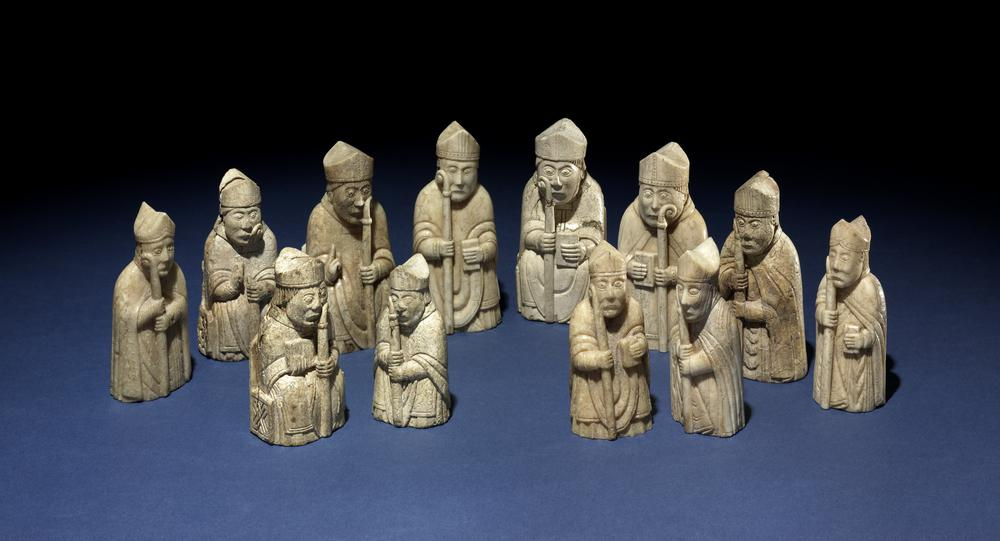
\includegraphics[width=0.5\textwidth]{chessmen}
        \caption{The Lewis chessmen are a group of distinctive 12th-century chess pieces, along with other game pieces, most of which are carved from walrus ivory. Present location: British Museum, London. Image courtesy of Wikipedia Commons}.
    \end{figure}

\section{Computing chess}




% Asa se specifica folosirea unui fisier cu referinte bibliografice:
\bibliographystyle{plain}
\bibliography{bibliography}

%\newpage


\end{document}